 \documentclass[11pt,a4paper]{report}
\usepackage[latin1]{inputenc}
\usepackage{csquotes}
\usepackage{amsmath}
\usepackage{mathtools}
\usepackage{pifont}
\usepackage{graphicx}
\usepackage{amsfonts}
\usepackage{amssymb}
\usepackage{fancyhdr}
\usepackage[left=4.5cm,right=4.5cm,top=4cm,bottom=2cm]{geometry}
\usepackage{listings}
\usepackage{color}
\usepackage{microtype}
\usepackage{booktabs}
\usepackage{chngcntr}
\usepackage{titlesec}
\usepackage{tikz}
\usepackage{float}
\usepackage{multicol}
\usepackage{multirow}
\usepackage{tikz-qtree}
\usepackage{pgftree}
\usepackage{caption}
\usepackage{subcaption}
\usepackage{algorithm}
\usepackage{algpseudocode}
\usepackage[export]{adjustbox}
\usepackage[final]{pdfpages}
\usepackage{float}
\usepackage{caption}
\usepackage[square,sort,comma,numbers]{natbib}
\usepackage[super,negative]{nth}
\usepackage{url}
\usepackage{dingbat}

                  
\usetikzlibrary{arrows, automata}

\setcounter{secnumdepth}{5}
\setcounter{tocdepth}{5}

\newcommand{\quotes}[1]{``#1''}
\newcommand{\at}{\makeatletter @\makeatother}
\newcommand{\HRule}{\rule{\linewidth}{0.5mm}} 
\pagestyle{fancy}%
  \renewcommand{\headrulewidth}{0.3pt}
  \renewcommand{\footrulewidth}{0pt}
  \renewcommand{\chaptermark}[1]{\markboth{#1}{}}
  \renewcommand{\sectionmark}[1]{\markright{#1}{}}
  \fancyhf{}
  \fancyhead[LE,RO]{\sffamily\bfseries\thepage}
  \fancyhead[LO]{\sffamily\bfseries\rightmark}
  \fancyhead[RE]{\sffamily\bfseries\leftmark}
  \fancyfoot{}
\renewcommand*\thesection{\arabic{section}}  

%\setcounter{secnumdepth}{5}
\counterwithin{paragraph}{subsubsection}
\counterwithin{subparagraph}{paragraph}

%\lstset{frame=shadowbox, rulesepcolor=\color{blue}}


\begin{document}

\pagenumbering{Roman} 

\begin{titlepage}
\begin{center}
{ \huge \bfseries \textbf{ Evaluating the performance of a new aligner for ultra-short ancient DNA }}\\[0.4cm]
\HRule \\[0.5cm]
% Author and supervisor
\begin{minipage}{0.9\textwidth}
\begin{flushleft} \large
{\textbf{Homa Amini}}\\
% Homa.Amini.0062\at student.uu.se\\
\end{flushleft}
\end{minipage}
%\begin{minipage}{0.4\textwidth}
%\begin{flushright} \large
%\emph{Supervisor:\\Janet Kelso}\\
%kelso\at eva.mpg.de
%\end{flushright}
%\end{minipage}
\vfill
% Bottom of the page
%{Create: \large Oct 2015}\\
%{Last update: \large \today}
\end{center}
\end{titlepage}

\newpage\null\thispagestyle{empty}\newpage
\newpage
\newpage

\section*{Abstract}

Recent technological developments, such as high-throughput sequencing,
have enabled the sequencing of the genomes of many living organisms.  
Recently, it has also become possible to extract and sequence DNA from 
extinct organisms.\\ 
In comparison with modern DNA, the computational analysis of ancient DNA
is complicated by the fact that the sequenced fragments tend to be short,
degraded and contaminated with extraneous environmental sequences, such 
as bacteria and modern human DNA.

Identification of endogenous sequences from this mix of DNA is generally
achieved by alignment to a reference genome sequence. However, existing 
alignment software does not work well with these ultra-short, chemically
damaged sequences.

In order to deal with these much older samples, a new software program 
has been implemented (R-Candy; U. Stenzel unpubl.)which aims to align 
these ultra-short reads and cope with the high levels of chemical damage 
present, using self-index data structures for pattern matching based on 
a Burrows-Wheeler Transform based FM-Index.

This thesis evaluates the accuracy and performance of the R-Candy aligner 
using simulated ancient DNA sequences. 

R-Candy is compared to BWA, which is currently the most-commonly used 
aligner for ancient DNA.

Tests on simulated data showed that R-Candy outperforms BWA (run using 
default and customized parameters), correctly aligning more endogenous 
reads correctly even in the presence of extensive deamination, as well
as incorrectly aligning fewer exogenous reads.

Future development of R-Candy will focus on increasing its speed by 
improving the search algorithm and adding support for multi-threading.

\newpage\null\thispagestyle{empty}\newpage
\section*{Acknowledgements}
\newpage\null\thispagestyle{empty}\newpage

\tableofcontents
\newpage
\listoftables
\newpage
\listoffigures
\newpage

\pagenumbering{arabic} 



\section{Introduction} \label{Introduction}


There have been a number of breakthroughs in the development of sequencing 
technologies that allow us to now sequence whole genomes rapidly and at a 
reasonable cost\cite{NGS}\cite{454}\cite{NGS2}.
\\
These developments made it possible to get DNA sequence from ancient 
organisms, including humans \cite{AncientDNA}\cite{fish2human}, and  
to learn about human history\cite{impactOFhg}\cite{ourGenome}\cite{SNP}.

Since the primary goal of many studies is to find the genetic 
relationships between extinct and extant species, most often sequences 
from ancient organisms are analysed by aligning them to the genomes of 
closely related extant species\cite{Neanthertal}\cite{AncientDNA}.

A number of problems have to be addressed when ancient DNA is aligned.
The continuous maintenance of a living organism by enzymatic repair stops 
shortly after a death of a living organism. Along with the action of
microbes, insects and fungi, this makes the extraction of a 
high-quality endogenous DNA very difficult and result in very short(the 
mean aDNA fragments vary between 36 to 150 base pairs providing by Illumina 
platform\cite{rizzi2012ancient} \footnote{This range varies due to environment 
and the age of the sample})and degraded DNA sequences\cite{paabo2004genetic}.
 
In addition, the degradation process of ancient DNA over time results 
in deamination of cytosine to uracil (and ??? are read as C to T 
changes) at the both ends of DNA fragments \cite{futureofaDNA}, the low amount 
of endogenous DNA that survived over a long period of time  
are highly contaminated \cite{paabo2004genetic}\cite{aDNA}by microbes.

For samples that are reasonably preserved approaches to the alignment
of reads that are longer than 35bps have been developed. 
These use standard alignment software (eg BWA) but modify the parameters 
to compensate more differences.
But for older or less well-preserved samples that have even shorter 
sequences $(<35 bps)$ \cite{meyer2014mitochondrial},
using standard aligners like BWA leads to incorrect alignments for a 
number of reasons.

First given the mammalian genome size, random alignments of shorter 
sequences become increasingly likely as the length decreases. 
This means that an increasing number of incorrect alignments can be 
found (and this is true for both endogenous and exogenous DNA).

Second, standard aligners don't include a model of chemical damage that 
is specific to ancient DNA, and, therefore, penalise reads with mismatches
that are due to chemical damage.

Third, most aligners require an exact match of some minimum length(seed), 
that is often longer than the read length possible with ancient DNA.

Therefore, due to the lack of proper tools such as an aligner that is 
specific to ancient data and its characteristics, much of the truly 
endogenous DNA may get discarded. A new aligner to efficiently analyze 
very poorly preserved ancient DNA would therefore be very useful.
\\
This thesis evaluates the performance of a new ancient DNA aligner,
R-Candy, and compares it with BWA which is a widely used aligner for
short reads.
<<<<<<< HEAD



=======



>>>>>>> ca3a198f381debd86dd87ad9edb9b768dbfde061
%%%%%%%%%%%%%%%%%%%%%%%%%%%%%%%%%%%%%%%%%%%%%%%%%%%%%%%%%%%%%%%%%%%%%%%%%%%%%%%%

\clearpage
\section{Background } \label{Background }


\emph{Sequencing} is the process of determining the precise order of bases 
(adenine, guanine, cytosine, and thymine) that compose a DNA molecule. 
It is typically very hard to sequence a long fragment of a DNA molecule, 
such as a whole chromosome. However, It is easy to subdivide longer sequences
into short pieces, create multiple copies of them (called \emph{amplification} ) 
and sequence all the copies. The sequence of every piece is called a read and 
the whole process is known as \emph{shotgun sequencing} \cite{algorithmDesign}.


The human genome sequence is made up of 3 billion DNA base pairs.
It is CpG poor and repeat-rich, 50\% of the human genome is consists 
of repetitive DNA sequences. The CpG sites are regions of DNA where 
a cytosine nucleotide is followed by a guanine nucleotide which are 
four folders under-represented in the human genome. Although it is 
completely sequenced but is not yet fully understood. 


%%%%%%%%%%%%%%%%%%%%%%%%%%%%%%%%%%%%%%%%%%%%%%%%%%%%%%%%%%%%%%%%%%%%%%%%%%%%%%%


\subsection{Ancient DNA } \label{Ancient DNA }

Ancient DNA reads can be broadly described the retrieval of DNA from fossils 
remains, archaeological discovery, museum specimens and other sources.

The extracted DNA from long-dead organisms has significantly different 
characteristics that distinguish it from modern DNA which are summarized in 
Table \ref{aDNAchar} .\\



\begin{table}[H]
  \begin{tabular}{ |  p{4cm} | p{2cm} | p{5cm} |}
    \hline
     \textbf{  Properties} & \textbf{Modern DNA } &\textbf{ ancient DNA} \\ \hline
     Molecule  length &  1000s of bps  & $\leq$  35 bps\\ \hline
     Post-Morten \hspace{35pt} substitutions & Few/low\hspace{35pt}frequency
     & Deamination of C$\to$T(more likely near the end of a read) \\ \hline
     Contaminated & negligible & exogenous+Modern human\\ \hline
  \end{tabular}
  \caption{Comparison between modern DNA and ancient DNA}
  \label{aDNAchar}
\end{table}


The challenges with ancient DNA was the requirement for new software to efficiently 
align millions of ultra-short, degraded and deaminated reads to a reference genome 
without being overwhelmed by spurious alignments of microbial contaminant reads.


\subsection{Alignment} \label{Alignment}

Sequence alignment is a common problem in computational biology, 
and one that can be simplified as follows:

An alignment between two strings $S_{1}$ and $S_{2}$ assumes a common origin and 
tries to highlight their similarities by explaining one of them as a small number 
of mutations, insertions and deletions applied to the other.\\

An alignment of two strings is a list of indices (i,j) where $S_{1}[i]$ matches
 $S_{2}[j]$.\\ 
In its simplest form an alignment of two strings is obtained by placing two strings
one above the other one in the way that every character in either string is above 
a unique character in opposite string and then looking for relation between them.\\\\

As an example, consider the alignment of two strings $S_{1}$:\emph{'CCGATGA'} 
and $S_{2}$:\emph{'TCGCTG'} shown below. 

\begin{center}
	%\begin{tabular}{c *{12}c|cc|c}
	\begin{tabular}{ c c c |c| c c |c|c| c c|c| c c}
%	\hline
   $S_{1}$   &  & & C & C & G & A & - & T & G & A && \\
	%\hline
$S_{2}$ 	&  & &{\textcolor{red}T}& C & G & {\textcolor{green}-}& {\textcolor{cyan}C } 
 &  T & G & {\textcolor{green}- }& \\
    	                                 
	\end{tabular}
\end{center} 
In this alignment,there is one mismatch of character T highlighted in red, 
two deletion of character A highlighted in green and one insertion of character
C highlighted in cyan and all the other characters match their counterparts in 
the opposite string. 
\\\\

There are some key issues for an ideal alignment that needs to be considered:

\begin{itemize} 
	\item  What sort of alignment.
	\item  What kind of scoring system.
	\item  What algorithm to find the optimal alignment score.
\end{itemize}




%%%%%%%%%%%%%%%%%%%%%%%%%%%%%%%%%%%%%%%%%%%%%%%%%%%%%%%%%%%%%%%%%%%%%%%%%%%%%%%

\subsubsection{The Scoring Model} \label{The Scoring Model}

Comparing two sequences, we need a score to measure their similarity.
In the case of biology, the assumption is that the two sequences differ
due to a mutation process that led to a substitution 
of one base by another base,as well as insertion and deletion (INDEL) which add or remove bases.
We are aiming at aligning the two sequences in a way that maximizes their similarity.\\ \\
First, let's set up the problem with some notation:\\
We call the two sequences, $S_{1}$ and $S_{2}$ of length N and M respectively. 
The $i^{th}$ symbol in $S_{1}$ is $S_{1i}$ and $j^{th}$ symbol in $S_{2}$ is $S_{2j}$. 
In the case of DNA, these symbols are $\left\{A, C, G, T\right\}$.\\
$S(S_{1i}, S_{2j})$ is the score of aligning $S_{1i}$ to $S_{2j}$ (match or mismatch)
and $\delta$ is a penalty for introducing a gap by insertion or deletion of a character. 
Then the score of an alignment will be the sum of the substitution scores minus the 
penalties in it(the scoring system for our alignment is described in section 3.2.1.5 in more details).\\\\
As an example, the following is the substitution matrix for DNA sequence alignments.


\begin{table}[H]
 \centering
  \begin{tabular}{  c| r  r r  r }
    
  \textbf{  $S(S_{1i}, S_{2j})$ } & \textbf{A} &\textbf{ C} &\textbf{ G} &\textbf{ T} \\ \hline
       \textbf{A} &  1  & -1 & -0.5 & -1 \\
       \textbf{C} & -1  & 1 & -1 & -0.5 \\ 
       \textbf{G} & -0.5 & -1 & 1 & -1 \\ 
       \textbf{T} & -1 & -0.5 & -1 & 1
    \end{tabular}
%\caption{comparation between modern DNA and ancient DNA}
\label{alignment-exp}
\end{table}

If $\delta$=1 then the total score of following alignment is:
 
\begin{center}
	\begin{tabular}{c *{12}cccc}
%	\hline
        & & C & C & G & A & - & T & A & G && \\
	%\hline
 	  & & T  & C & G &  -  & C   &  T & -  & G & \\
    	                                 
	\end{tabular}
\end{center} 

-0.5 + 1 + 1 - 1 - 1 + 1 - 1 + 1 = 0.5



%%%%%%%%%%%%%%%%%%%%%%%%%%%%%%%%%%%%%%%%%%%%%%%%%%%%%%%%%%%%%%%%%%%

\subsubsection{Alignment Algorithms} \label{Alignment Algorithms}
Having the scoring system, we need an algorithm for finding the 
optimal alignment between a pair of sequences. 
Aligning a sequence of length N to another sequence of length N,
there is only one global alignment but things get complicated when 
gaps are allowed.
 
There are \cite{durbin}
$$ \binom{2n}{n} = \frac{(2n)!}{(n!)^2} \simeq \frac{2^{2n}}
{\sqrt{2\pi n}} $$
global alignments between two sequences of length N.

Obviously, it is not computationally doable to calculate all these
alignments. Therefore, finding the optimal alignment between two 
sequences is a crucial part in computational sequence analysis.
Such an algorithm is called dynamic programming, which uses an 
additive alignment score for  weighting alignments. 

For different types of alignment, there are slightly different 
types of dynamic programming algorithms (alignment algorithms).\\\\


The four essential steps in all dynamic programming algorithms are:

\begin{itemize} 
	\item Define a recursive structure for the optimal score
	\cite{eddydynamic}.
	\item  Create a  matrix for remembering the optimal score 
	of subproblems \cite{eddydynamic}.	
	\item Fill the matrix by solving the  subproblems in a 
	bottom-up approach\cite{eddydynamic}.
	\item Reconstruct the optimal approach that led us to the 
	optimal score by a traceback on the matrix\cite{eddydynamic}.
\end{itemize}

In the following part I will describe the three more basic alignment 
algorithms that easily can be expanded to the more complex versions.




%%%%%%%%%%%%%%%%%%%%%%%%%%%%%%%%%%%%%%%%%%%%%%%%%%%%%%%%%%%%%%%%%%%%%

\paragraph{ Global alignment (Needleman-Wunsch algorithm) }

The Needleman-Wunsch algorithm, which is based on dynamic programming, 
is an established global alignment technique in biological 
sequence analyses to obtain the best-matching alignment of two sequences, 
allowing  gaps.\\
It aims to construct an optimal alignment using previous solutions for
optimal alignments of smaller subsequences \cite{durbin}.\\
We are going to calculate the optimal alignment score as been described 
in\cite{durbin} by constructing a matrix $F$ indexed
by $i$ and $j$, one index for each sequence, where the value $F(i, j)$ is the score
of the best alignment between the initial segment $S_{1\{1..i\}}$ of $S_{1}$ 
up to $S_{1i}$ and the initial segment $S_{2\{1..j\}}$ of $S_{2}$  up to 
$S_{2j}$. We can build $F(i, j)$ recursively start by initialising 
$F(0, 0) = 0$. Afterwards we fill the matrix matrix from top left to 
bottom right. 
Once $ F(i-1, j-1 ), F(i-1 , j) $ and $ F(i , j-1) $ are known, we 
are able to calculate $ F(i, j)$ \cite{durbin}.

The best score of $F(i,j)$ up to $S_{1i}$ and $S_{2j}$ is the maximum 
value of $S(i,j)$:

\[ F(i,j)= \max
\begin{cases}
   F(i-1,j-1) + S(S_{1i} , S_{2j})\\
   F(i-1 , j)- \delta\\
   F(i,j-1)- \delta
\end{cases}
\]
The value in the last cell of matrix $F(n,m)$ is by definition the optimal 
alignment score. 
For obtaining the alignment itself we need the path that led us to the 
final score. We use the trace back procedure to recursively recover the 
optimal alignment\cite{durbin}\cite{eddydynamic}.
We start from the last cell $F(n,m)$ and follow each of the three cases 
that we chose to get to this point. We continue doing this until reaching
the cell $F(0,0)$ and in this point the optimal alignment is completely 
reconstructed \cite{eddydynamic}.




%%%%%%%%%%%%%%%%%%%%%%%%%%%%%%%%%%%%%%%%%%%%%%%%%%%%%%%%%%%%%%%%%%%%%%%%%%%

\paragraph{ Local alignment (Smith-Waterman algorithm) }

Compute the maximum scoring alignment of $L(S_{1}, S_{2})$ over all 
sub-sequences $S_{1}$ and $S_{2}$ is:


\[ F(i,j)= \max
\begin{cases}
   F(i-1,j-1) + s(S_{1i} , S_{2j})\\
   F(i-1 , j)+ \delta\\
   F(i,j-1)+ \delta\\
   0 \quad  
\end{cases}
\]

To find the actual local alignment:
\begin{itemize}
 \item start at a cell with the maximum value.
 \item traceback.
 \item stop when you reach a cell with value 0.
\end{itemize} 





%%%%%%%%%%%%%%%%%%%%%%%%%%%%%%%%%%%%%%%%%%%%%%%%%%%%%%%%%%%%%%%%%%%%%%%%%%%%%%%%%%%%%%

\paragraph{Semi-global alignment}

Semi-global or "glocal" (short for global-local) algorithm is a combination 
of global and local alignments. 
It is a practical strategy in the case of ancient DNA.
Aligning two sequences, one short (an ancient DNA read) and the 
other one long (a chromosome sequence). In this case, neither global 
nor local alignment is completely applicable. The best solution here 
is to globally align the short sequence while only a local alignment
is appropriate for the long sequence.


Having two sequences  $S_{1}$ and $S_{2}$, want to optimally align them.
$$S_{1}:ACACACTACCG$$
$$S_{2}:AGCACACA$$\\

\[ F(i,j)= \max
\begin{cases}
   s(S_{1i},S_{2j})= +2 \quad \mbox{match} \\
   s(S_{1i},S_{2j})= -1 \quad \mbox{mismatch} \\
  \delta = -1  \quad \mbox{gap penalty} \\ 
\end{cases}
\] \\



$
H =\left
[
\begin{array}{ *{13}c} 
   & $\_$ & A & C & A & C & A & C & T & A & C & C & G \\
 $\_$  & \textcolor{cyan}{0} & 0 & 0 & 0 & 0 & 0 & 0 & 0 & 0 & 0 & 0 & 0 \\
 A & 0 & \textcolor{cyan}{2} & 1 & 2 & 1 & 2 & 1 & 1 & 2 & 1 & 0 & 0 \\
 G & 0 & \textcolor{cyan}{1} & 1 & 1 & 1 & 1 & 1 & 0 & 1 & 1 & 0 & 2 \\
 C & 0 & 1 & \textcolor{cyan}{3} & 2 & 3 & 2 & 3 & 2 & 1 & 3 & 3 & 2 \\
 A & 0 & 2 & 2 & \textcolor{cyan}{5} & 4 & 5 & 4 & 3 & 4 & 3 & 2 & 2 \\
 C & 0 & 1 & 4 & 4 & \textcolor{cyan}{7}  & 6 & 7 & 6 & 5 & 4 & 5 & 4 \\
 A & 0 & 2 & 3 & 6 & 6 & \textcolor{cyan}{9} & 8 & 7 & 8 & 7 & 6 & 5 \\
 C & 0 & 1 & 4 & 5 & 8 & 8 & \textcolor{cyan}{11} & \textcolor{cyan}{10} & 9 & 10 & 9 & 8 \\
 A & 0 & 2 & 3 & 6 & 7 & 10 & 10 & 10 & \textcolor{red}{12} & 11 & 10 & 9 \\
 \end{array} 
 \right]
$\\\\\\
Filling the matrix, the optimal alignment score will be the largest value
in the entire array.\\\\


$
T =\left
[ 
 \begin{array}{ *{13}c} 
       & $\_$ & A & C & A & C & A & C & T & A & C & C & G\\
  $\_$ & \textcolor{black}{0} & 0 & 0 & 0 & 0 & 0 & 0 & 0 & 0 & 0 & 0 & 0 \\
 A & 0 & \textcolor{red}{\nwarrow} & \leftarrow & \nwarrow & \leftarrow & \nwarrow & \leftarrow & \leftarrow & \nwarrow & \leftarrow & \leftarrow & \leftarrow \\
 G & 0 & \textcolor{red}{\uparrow} & \nwarrow & \uparrow & \nwarrow & \uparrow & \nwarrow & \nwarrow & \uparrow & \nwarrow & \leftarrow & \nwarrow \\
 C & 0 & \uparrow & \textcolor{red}{\nwarrow} & \leftarrow & \nwarrow & \leftarrow & \nwarrow & \leftarrow & \leftarrow & \nwarrow & \nwarrow & \leftarrow \\
 A & 0 & \nwarrow & \uparrow & \textcolor{red}{\nwarrow} & \leftarrow & \nwarrow & \leftarrow & \leftarrow & \nwarrow & \leftarrow & \leftarrow & \nwarrow \\
 C & 0 & \uparrow & \nwarrow & \uparrow & \textcolor{red}{\nwarrow} & \leftarrow & \nwarrow & \leftarrow & \leftarrow & \leftarrow &  \nwarrow & \nwarrow \\
 A & 0 & \nwarrow & \uparrow & \nwarrow & \uparrow & \textcolor{red}{\nwarrow} & \leftarrow & \leftarrow & \nwarrow & \leftarrow & \leftarrow & \leftarrow\\
 C & 0 & \uparrow & \nwarrow & \uparrow & \nwarrow & \leftarrow & \textcolor{red}{\nwarrow} & \textcolor{red}{\leftarrow} & \leftarrow & \nwarrow & \leftarrow & \leftarrow \\
 A & 0 & \nwarrow & \uparrow & \nwarrow & \uparrow & \nwarrow & \uparrow & \nwarrow & \textcolor{red}{\nwarrow}  & \leftarrow & \leftarrow & \leftarrow \\
 \end{array} 
\right]
$\\\\\\
The red path corresponds to the semi-global alignment of the two 
sequences $S_{1}$ and $S_{2}$: 
$$S_{1}:A-CACAC\enskip TACCG$$
$$S_{2}:A\enskip G CACAC-A\enskip\enskip\enskip\enskip\enskip $$



Semi-global\footnote{Reads are globally aligned (fully aligned) 
where the reference is locally aligned (with some gaps at the 
end of the reference string)} alignments are produced 
by R-Candy as a result of mapping sets of short queries against 
a long reference sequence (for instance, aligning queries of 
length 25-50 bps to the human reference genome of length 3.2 Gbps).

It would be possible to determine the best alignment by filling a 
scoring matrix and tracing it back, however filling the dynamic 
programming scoring matrix for a reference sequence of mammalian 
size genome is costly as the time complexity is proportional to 
the length of the reference genome. Therefore, R-Candy uses a 
Full-Text index for its alignment strategy instead of dynamic 
programming. 


%%%%%%%%%%%%%%%%%%%%%%%%%%%%%%%%%%%%%%%%%%%%%%%%%%%%%%%%%%%%%%%%%%%%%%%%%%%%%%%% 

\paragraph{Scoring for ancient DNA} \label{Scoring}


Specifically for ancient DNA, we treat damage by the following
adaptations of the general scoring scheme.\\
A DNA molecule read is thought of as composed of two single-stranded parts at 
the 3' and 5' terminals (called ``overhang parts'') and a 
double-stranded stem for non-overhang parts (the middle part of
a read). From knowledge of the chemistry of DNA\cite{DNAchemistry}, high rates 
of nucleotide misincorporation as a result of \emph{post-mortem} 
deamination damage on the overhang parts of aDNA reads are assumed, and
the length of the overhangs is approximately 
geometrically distributed\cite{mapdamage2}. 

Let $\sigma$ and $\delta$ be the single stranded and the double stranded
deamination rates.  Let $l$ be the length of the read being aligned.  

For single stranded library preparation, let $\lambda_s$, $\kappa_s$ be
the 5' overhang length parameter and the 3' overhang parameter.  Let $l$
be the length of the read being aligned.  For every position $i \in
[0..l-1]$ define

\begin{align*}
p_{\mbox{fwd}} &= \lambda_s^{i+1} + \kappa_s^{l-i} - \lambda_s^{i+1} \kappa_s^{l-i} \\
p_{\mbox{rev}} &= 0
\end{align*}

Now define effective substitution probabilities

\begin{equation*}
p_{C} = \sigma p_{\mbox{fwd}} + \delta (1 - p_{\mbox{fwd}}), \quad
p_{G} = \sigma p_{\mbox{rev}} + \delta (1 - p_{\mbox{rev}}) 
\end{equation*}

Scoring a base at position $i$ with quality score $q$ involves
deamination, divergence and error.  We assume both a trivial error model
and a trivial model of evolution, where all possible changes occur with
a uniform rate derived from the quality score and a uniform rate given
by parameter $D$, respectively.  Define 

\begin{equation*}
\epsilon_0 = {10^{-q/10}}/4, \quad \epsilon = \epsilon_0 + D/3 - \epsilon_0 D/3
\end{equation*}

and the complete substitution matrix becomes (with the reference base in
columns and the
query base in rows, both in the order A, C, G, T):

\begin{equation*}
\left( \begin{array}{cccc}
1 - 3 \epsilon &       \epsilon                            &       \epsilon + p_{G} - 4 \epsilon p_{G} &       \epsilon \\
      \epsilon & 1 - 3 \epsilon - p_{C} + 4 \epsilon p_{C} &       \epsilon                            &       \epsilon \\
      \epsilon &       \epsilon                            & 1 - 3 \epsilon - p_{G} + 4 \epsilon p_{G} &       \epsilon \\
      \epsilon &       \epsilon + p_{C} - 4 \epsilon p_{C} &       \epsilon                            & 1 - 3 \epsilon 
\end{array} \right)
\end{equation*}

Alignment scores are the sum of the natural logarithms of the
entries in that matrix for every aligned base, plus a penalty for
insertions and deletions.  We use linear gap costs with a cost of $G$
per inserted or deleted base, where $G$ is another parameter.



%%%%%%%%%%%%%%%%%%%%%%%%%%%%%%%%%%%%%%%%%%%%%%%%%%%%%%%%%%%%%%%%%%%%%%%%%%%%%%%

\subsection{Data Structures}  \label{Data Structures}

Some of the main data structures used by our new aligner (R-Candy)
for indexing and mapping process plus fundamental concepts required
for better understanding of this thesis are described in this section. 



%%%%%%%%%%%%%%%%%%%%%%%%%%%%%%%%%%%%%%%%%%%%%%%%%%%%%%%%%%%%%%%%%%%%%%%%%%%%%%%%%%%%%%%

\subsubsection{Preliminaries} \label{Preliminaries}

\begin{table}[h]
 \centering
  \begin{tabular}{ | p{0.5cm} | p{0.5cm} | p{0.5cm} 
  |p{0.5cm} |p{0.5cm} |p{0.5cm} |p{0.5cm} |p{0.5cm} |}
    \hline
  \textbf{b} & \textbf{a } &\textbf{r}  &\textbf{b} 
  &\textbf{a} &\textbf{r} &\textbf{a} &\textbf{\$}\\ \hline
       0 & 1 &2&3&4&5&6&7 \\ \hline
      
   \end{tabular}
\caption{Array representation of "barbara" string}
\label{Array-representation}
\end{table}



A string \emph{S} is concatenation of \emph{N} characters. 
The length of the \emph{S} is denoted as $\lvert S \rvert$ 
= N and S[i] represents the $i_{th}$ character of the S.
The string's index starts from 0 and S[0,N-1] represents 
the whole string S while S[i..k] shows the substring of S 
from the position i to k inclusive with $i < k < N$. 
S[i..N-1] is the i\textsuperscript{th} suffix of So the 
2th suffix of above example is S[2..7]='arbara\$' and
S[0..i] is defined as i\textsuperscript{th} prefix, so 
the 7\textsuperscript{th} of table 2 is 'barbara\$'.
The pattern that we will be searching for is P.

$ \sum $  denotes the alphabet that all the characters of 
S belong to it And $ c_{i} < c_{k}$ means $c_{i}$ appears 
before $c_{k}$ in lexicographic ordering.

A genome is presented by four letters $\left\{ 'A', 'C', 
'G' and\,'T'\right\}$, which corresponds to adenine, cytosine, 
guanine and thymine nucleotides. The character ('N') usually 
represents positions that are unknown in a genome.



%%%%%%%%%%%%%%%%%%%%%%%%%%%%%%%%%%%%%%%%%%%%%%%%%%%%%%%%%


\subsubsection{Suffix Trie and R-Candy's Alignment Algorithm} 
\label{Suffix Trie and R-Candy's Alignment Algorithm}

A Trie is a rooted tree data structure with labeled edges 
by letters in the alphabet and nodes with concatenated 
characters from the root\cite{trie}.\\ 
A Trie of all the suffixes of string S is called a Suffix 
Trie where each path from the root to a leaf is a suffix 
\cite{gusfield1997algorithms}.
The memory consumption of a Suffix Trie at the worst case 
for a genome of length n is  $\mathcal{O} (n^{2})$.
\\\\

R-Candy uses a suffix Trie as its abstract data structure
and Depth First Search (DFS) on the Trie as its alignment algorithm.
Although its index structure is an FM-Index but it is simulated as a Trie.

A query gets aligned to a reference tree where a top-down traversal
of the tree's branches is a Depth First Search of a query alignment.

R-Candy applies a semi-global alignment, where queries 
align globally and  references locally.

In a top-down traversal of the suffix Trie for every node, the 
minimum score of match$/$mismatch, insertion and deletion between
two characters is chosen.It means trying a different branch for 
every INDEL, which yields a very big number. Fixing this problem 
R-Candy allows just one INDEL per alignment, which in the case
of aDNA with very short reads, is very practical and saves a lot of
time and memory. It tries one branch that runs down all the suffixes
that are at least as long as the query even though it has a big 
number of mismatches which is pointless and that's a bound which is
the maximum score that we are willing to endure and puts a filter on
branching which is a cutoff value based on practical reasons and gets
into the program as an alignment score parameter. In practice, it starts
with the AS limit if searches for an alignment, if can not reports no 
alignment found and if finds some alignments lowers the limit and repeats 
the process calling it branch and bound algorithm. When the query is 
totally aligned, the alignment is done, no matter just a small part of 
the reference is aligned.
\\\\
Given a non-empty sequence $q\in (q_{1}..q_{n})$, we want to align it to 
another non-empty sequence (reference)$r\in (r_{1}..r_{n})$.\\
In the top-down traversal of tree branches for each character 
of queries ($q_{i}$) the minimum score of three options match or mismatch, 
insertion and deletions, of $q_{i}$  and the labeled character ($r_{i}$)
on the tree branch is calculated as described in the following pseudocode.
For each new alignment of ($q_{i}$) and ($r_{i}$), the score will be the
computed score so far plus match score with Match operation (M) in the 
CIGAR field \cite{samtools} for match case. In the case of insertion (I) 
it will be the calculated score so far plus insertion score (penalty) pair 
with insertion operation and CIGAR field for insertion.
The same procedure applies to the case of deletion.
Notice that this algorithm is not DP and therefore will
perform badly if multiple gaps are necessary.\\


\begin{lstlisting}[language=Haskell, basicstyle=\ttfamily\scriptsize, 
keywordstyle=\color{red}, frame=single ]

go lim score node k _ | score > lim = k lim
go lim score node k [      ] = (node, score) : k (min lim score)
go lim score node k (pp:pps) =
    go' lim $ sortBy (comparing fst) $
        ( gapscore, \l' s' k' -> go l' s' node k' pps ) :                   
        [ ( pp ! sym, \l' s' k' -> go l' s' node' k'     pps  )
            | (sym,node') <- children node ] ++
        [ ( gapscore, \l' s' k' -> go l' s' node' k' (pp:pps) ) 
            | (sym,node') <- children node ]
  where
    go' l [          ] = k l
    go' l ((ds,k'):xs)
        | score' > l = k l               
        | otherwise  = k' l score' (\l' -> go' l' xs)
      where score' = score + ds

\end{lstlisting}



But the alignment can be much faster by using \emph{seed} 
heuristic. 
Many programs (e.g. BWA) reduce the amount of backtracking  
by dedicating the first part of the read as a seed 
\footnote{ Set a limit on the number of allowed mismatches 
in the first few tens of bases on a read sequence, is called
the \emph{seed} sequence.}and allowing fewer mismatches in 
the seed portion \cite{bwa}. By default, BWA uses the first 
32 bps of a read sequence as a seed, allowing maximum two 
mismatches in order to increase the overall speed of the 
alignment (for reads that are shorter than 32 bps, the seed 
is disabled)\cite{bwa}. 

But the beginning part of the read can not serve as a seed
because the beginning part of aDNA reads are damaged,
but the middle part could if a middle-out mapping strategy
was implemented.



%%%%%%%%%%%%%%%%%%%%%%%%%%%%%%%%%%%%%%%%%%%%%%%%%%%%%%%%%%%%%%%%%%%%%%%%%%%%%%%%%

\subsubsection{Suffix Tree and Suffix Array}
\label{Suffix Tree and Suffix Array}

Coalescing each non-branching path of a Suffix Trie into 
a single edge, labeled by the string of that path, namely 
Suffix Tree reduces the memory complexity to $\mathcal{O}(n)$.
But the big-O notation ignores a big constant overhead 
of \~20 of the best known implementation of a Suffix Tree
\cite{gusfield1997algorithms}.\\ 


Suffix Array was developed by Manber and Myers(1990) in order to reduce the 
memory requirement of suffix tree. In other words Suffix Array is a compact 
representation of Suffix Tree. \\
A suffix array for a string S[1..k], can be constructed like:
\begin{itemize} 
	\item  Construct all the suffixes of string S.
	\item  Alphabetically sort all these strings.
	\item Store all the starting indices of all these suffixes.
\end{itemize}
Figure 4 shows the construction of suffix array for string "barbara".
\begin{figure}[H]
\centering
\begin{subfigure}{.2\textwidth}
%  \centering
  %\includegraphics[width=.4\linewidth]
\textbf{SA}  \\
\enspace  \textbf{0}\quad barbara\$\\
\textbf{1}\quad arbara\$\\
\textbf{2}\quad rbara\$\\
\textbf{3}\quad  bara\$\\
\textbf{4}\quad   ara\$\\
\textbf{5}\quad     ra\$\\
\textbf{6}\quad     a\$\\
\textbf{7}\quad       \$
  \caption{All suffixes of string S}
  \label{fig:sub1}
\end{subfigure}%
\begin{subfigure}{.2\textwidth}
 % \centering
\textbf{$\xrightarrow{sort}$}
\label{fig:sub1}
\end{subfigure}%
\begin{subfigure}{.3\textwidth}
%  \centering
%  \includegraphics[width=.4\linewidth]{image1}
\textbf{SA} \\
\textbf{7}\quad \$\\
\textbf{6}\quad a\$\\
\textbf{4}\quad ara\$\\
\textbf{1}\quad arbara\$\\
\textbf{3}\quad bara\$\\
\textbf{0}\quad barbara\$\\
\textbf{5}\quad ra\$\\
\textbf{2}\quad rbara\$
 \caption{sorted  Lexicographically.}
  \label{fig:Burrows-Wheeler transform}
\end{subfigure}
\caption{Suffix array for string "barbara".}
\label{fig:test}
\end{figure}


Since nodes of the Suffix Trie corresponds to ranges in the Suffix 
Array, therefore the Suffix Array serves as a replacement for 
the Suffix Trie.


%%%%%%%%%%%%%%%%%%%%%%%%%%%%%%%%%%%%%%%%%%%%%%%%%%%%%%%%%%%%%%%%%%%%%%%%%%%%%%%

\subsubsection{The Burrows-Wheeler Transform} 
\label{The Burrows-Wheeler Transform}


The Burrows-Wheeler Transform (BWT) is a text transformation data structure, 
with fast search query times and efficient memory consumption, which makes 
it very efficient at data compression. In this section, the construction scheme
of BWT and its relation with Suffix Array is described.\\


%%%%%%%%%%%%%%%%%%%%%%%%%%%%%%%%%%%%%%%%%%%%%%%%%%%%%%%%%%%%%%%%%%%%%%%%%%%%%%%

\paragraph{Construction and Properties}

A Burrows-Wheelers transformation for a string S[0..L] is s special rearrangement 
of its characters into substrings of the same characters (run) called $S^{BWT}$ 
and consists of the following steps \cite{bwt}:

\begin{itemize} 
	\item Append special character \$ as a terminator symbol to the end of S 
	which assume to be lexicographically smaller than any other alphabet 
	characters.
	\item  Construct all the cyclic rotations of S.
	\item  Sort them Lexicographically.
	\item The last column of this conceptual matrix \emph{$M_{T}$}, is called 
	BWT ( transformed text $S^{BWT}$ ).
\end{itemize}


For example, the BWT of string "barbara" is "arbbr\$aa", as shown in Figure 
\ref{barbaraBWT}.\\



\begin{figure}[H]
\centering
\begin{subfigure}{.5\textwidth}
  \centering
barbara\$\\
\$barbara\\
a\$barbar\\
ra\$barba\\
ara\$barb\\
bara\$bar\\
rbara\$ba\\
arbara\$b
%}
  \caption{All cyclic rotations for 'S'}
  \label{fig:barbaraBWT1}
\end{subfigure}%
\begin{subfigure}{.1\textwidth}
  \centering
$\xrightarrow{sort}$
\label{fig:sub1}
\end{subfigure}%
\begin{subfigure}{.5\textwidth}
  \centering
%  \includegraphics[width=.4\linewidth]{image1}
\$barbar\textcolor{red}{a}\\
a\$barba\textcolor{red}{r}\\
ara\$bar\textcolor{red}{b}\\
arbara\$\textcolor{red}{b}\\
bara\$ba\textcolor{red}{r}\\
barbara\textcolor{red}{\$}\\
ra\$barb\textcolor{red}{a}\\
rbara\$b\textcolor{red}{a}
 \caption{sorted  Lexicographically.}
  \label{fig:Burrows-Wheeler transform}
\end{subfigure}
\caption{Burrows-Wheeler transform for "barbara" string.}
\label{barbaraBWT}
\end{figure}




\begin{table}[h]
 \centering
  \begin{tabular}{ | p{0.5cm} | p{0.5cm} | p{0.5cm} |p{0.5cm} 
  |p{0.5cm} |p{0.5cm} |p{0.5cm} |p{0.5cm} |}
    \hline
  \textbf{a} & \textbf{r} &\textbf{b}  &\textbf{b} &\textbf{r} 
  &\textbf{\$} &\textbf{a} &\textbf{a}\\ \hline
       0 & 1 &2&3&4&5&6&7 \\ \hline
      
   \end{tabular}
\caption{Burrows-Wheelers transform of "barbara" string}
\label{BWT-barbara}
\end{table}



The first property of BWT is its special relationship with Suffix 
Array as described below: \\\\
Let SA[i] denote the suffix at 0-based offset \emph{i} in SA(S)
and BWT[i] denote the character at 0-based offset \emph{i} in 
BWT(S), as can be seen in Table \ref{BWT&SA}\cite{bwt}.\\


\[ f(n)
\begin{cases}
    BWT[i]=S[SA[i]-1]   & \quad \text{if } SA[i] > 0\\
    \$  & \quad \text{if } SA[i]= 0\\
\end{cases}
\]


\begin{table}[h]
\centering
  \begin{tabular}{ c c l}
%  \begin{tabular}{| m{23pt} | m{23pt}| m{23pt}|}
  \textbf{  BWT} & \textbf{SA } & \\ 
       a 	&	 7	 &   \$\\  
       r 	&	 6	 &	 a\$ \\
       b 	&	 4	 &	 ara\$ \\
       b 	&	 1	 &	 arbara\$ \\
       r  	&	 3	 &	 bara\$ \\
      \$ 	&	 0	 &	 barbara\$ \\
       a 	&	 5	 &	 ra\$ \\
       a 	&	 2	 &	 rbara\$ \\

  \end{tabular}
  
\caption{The relation between BWT and SA}
\label{BWT&SA}
\end{table}

Constructing all the cyclic rotations of a string S and sorting 
them is time and memory consuming. 
Therefore by using this property (the relation between SA and 
$S^{BWT}$ ), is possible to construct the $S^{BWT}$ directly 
from the SA of S.
\\\\
The second useful property of BWT is the last to first mapping.\\\\
\textbf{LF-mapping}  Last to first mapping describes the relation 
between the last(L) and first(F) column of $M_{T}$\cite{bwt}.\\\\
\textbf{Lemma 1:}\emph{the $i^{th}$ occurrence of c in the first 
column \emph{F} corresponds to the $i^{th}$ occurrence of the symbol 
c in the Last column \emph{L} of $M_{T}$} \cite{bwt}.\\\\
Figure \ref{Lemma1} illustrates Lemma 1\\

\begin{figure}[H]
\centering
\textcolor{cyan}{\$}barbar\textcolor{red}{$a_1$}\\
\textcolor{red}{$a_1$}\$barba\textcolor{green}{$r_1$}\\
\textcolor{red}{$a_2$}ra\$bar\textcolor{blue}{$b_1$}\\
\textcolor{red}{$a_3$}rbara\$\textcolor{blue}{$b_2$}\\
\textcolor{blue}{$b_1$}ara\$ba\textcolor{green}{$r_2$}\\
\textcolor{blue}{$b_2$}arbara\textcolor{cyan}{\$}\\
\textcolor{green}{$r_1$}a\$barb\textcolor{red}{$a_2$}\\
\textcolor{green}{$r_2$}bara\$b\textcolor{red}{$a_3$}
 \caption{Last to first property of BWT matrix}
 \label{Lemma1}
\end{figure}

A \emph{prefix\_sum table}(C) and an \emph{occurrence table}
(OCC) are required to comprehend LF-mapping in an efficient time 
complexity of \emph{O(1}).\\

\begin{itemize}

	\item C[c] is a table that for each character in 
	the alphabet contains the total number of text 
	characters that are alphabetically smaller than
	 \emph{c} \cite{fmindex}.

	
	\item OCC(c,q) denotes:  The total number of 
	occurrences of character c in the prefix 
	L[1..q]\cite{fmindex}.It is possible to 
	compute OCC(c, q) in constant time.
	
\end{itemize}

Using \emph{OCC} and \emph{C}, the LF-mapping 
is determined as follow
$$\emph{LF(i) = C[L[i]] + OCC(L[i], i)}$$ \\\\

As an example, for $S^{BWT}$ = "arbbr\$aa", the LF-mapping
for the first 'a' is OCC('a',0)+C('a')= 0 + 1 = 1, which is 
the position of 'a' in the first column (F).



%%%%%%%%%%%%%%%%%%%%%%%%%%%%%%%%%%%%%%%%%%%%%%%%%%%%%%%%%%%%%%%%%%%%%%%%%%%%%%%


\paragraph{Reversing} \label{Reversing}

We can use the LF-mapping on $S^{ BWT}$ to reconstruct the original string. 
Reconstructing the original string using the described features and prefix-sum
and occurrence tables is feasible by a backward reconstruction. As an example, 
retrieving the S="barbara" using its $S^{BWT}$= "arbbr\$aa" using Figure 
\ref{Lemma1} is achieved as follow.Starting with \$ symbol on the first row, 
knowing if we go backward the character before \$ is $a_1$ and also using 
LF-mapping. We know $a_1$ has the same position as $a_1$ in the first column of
the second row. Continuing backward hit $r_1$. Apply the LF-mapping principle 
again and say this is the first occurrence of r, then we go to the  $r_1$ in 
the first column of $7^{th}$ row and continue using the LF-mapping and then walk
back one step and so on. We reconstructed the original string in reverse. 
The memory requirement for BWT decompression is $\mathcal{O}(\lvert 1 \rvert)$ \\
<<<<<<< HEAD


=======


>>>>>>> ca3a198f381debd86dd87ad9edb9b768dbfde061
%%%%%%%%%%%%%%%%%%%%%%%%%%%%%%%%%%%%%%%%%%%%%%%%%%%%%%%%%%%%%%%%%%%%%%%%%%%%%%%%

\paragraph{Searching}

Generally, the searching algorithm for a pattern using $S^{BWT}$ is close to
the reversing procedure explained in the last Section. Recalling that suffixes 
with the same prefix are adjacent in the SA of S, we divide the searching procedure 
into two parts, the counting and localizing.\\


\textbf{Counting}

The BWT matrix is constructed by sorting all the cyclic rotations of a string, 
therefore if a pattern \emph{P} appears in the string it will be a prefix in $M_{T}$ 
and if \emph {P} appears in multiple positions, they will be successive. To search 
for a pattern using $S^{BWT}$, the backward search starts from the end of a pattern.
At first searches for an empty  pattern all over the BWT matrix. Then looks for the 
last character of the desired pattern. After finding the character, updates indexes 
and search for the character before that last one among the updated indexes.
Continues the process to find the pattern. Updating indexes is the crucial part 
of this procedure (See Figure \ref{backwardSearch}).\\\\


\begin{algorithm}[H]
   \caption{BWT backward search algorithm for a 
   given character c $\in \sum $ and an 
   $\omega$-range [i..j]}
   
    \begin{algorithmic}[1]
      \Function{backwardSearch}{$c ,[i..j]$}
       	\State ${i \leftarrow C[c] + OCC(c, i-1)+1}$
        \State ${j \leftarrow C[c] + OCC(c,j)}$
        	\If{$ i \leq j$} 
        		\State \textbf{return} [i..j]
        	\Else
        		\State \textbf{return} $\perp$
        	\EndIf 
    \EndFunction

	\end{algorithmic}
  \label{backward search alg}	
\end{algorithm}




\begin{figure}[H]
\centering
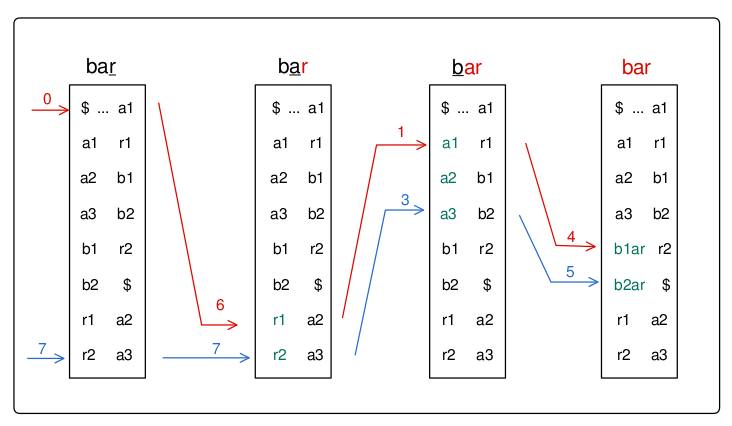
\includegraphics[width=12cm]{pictures/bar_1.png}
\caption{Backward search for pattern "bar" in 
string S using first and 
last column of BWT matrix. Updating indexes 
iteratively.}
\label{backwardSearch}
\end{figure}


\textbf{Locating} \label{Locating}

In the counting process, using backward search, we determine a range in SA of S
that points to the occurrences of a pattern in the string S. Hence these entries
in the SA reveal the matching position of a pattern in the string S.\\

\textbf{Time Complexity} 
The running time of the backward search on BWT depends on two factors; the length 
of the pattern P and more importantly, the access time of P in the suffix array.\\
The search algorithm consists of two phases, counting the number of occurrences 
of a pattern and localization of their positions in the string. The counting time 
is linear to the length of the P , assuming OCC table is implemented in a constant
time and the length of the string doesn't have any impact on searching time which 
is one of the main reasons of using BWT for a large string like a genome. On the 
other hand, the localization time is more affected by the number of occurrences of 
the pattern  because, for each occurrence of P, a look up at SA is needed.

The BWT of the reverse reference genome constructed by R-Candy simulates a Suffix 
Trie with nodes corresponding to ranges in BWT. Therefore, the LF-mapping of BWT 
applies a forward search on the Suffix Trie.

After introducing BWT and its properties and emphasizing on its important job in 
pattern searching, in the following section the usage of BWT in an indexing data 
structure called FM-Index will be discussed\cite{fmindex}. 


%%%%%%%%%%%%%%%%%%%%%%%%%%%%%%%%%%%%%%%%%%%%%%%%%%%%%%%%%%%%%%%%%%%%%%%%%%%%%%%

\subsubsection{FM-Index (Full-text index)}  
\label{FM-Index (Full-text index)}


Paolo Ferragina and Giovanni Manzini in 2000, six years after BWT was 
published invented a self-index data structure that combines BWT with 
some small auxiliary data structures. It allows to efficiently search 
for the occurrences of an arbitrary pattern P as a substring of the 
string S as well as localizing the position of each occurrence. They 
named it FM-Index for Full-Text Index in minute space where minute 
space emphasises on its memory efficiency of $\mathcal{O}(\lvert n 
\rvert)$ .The FM-Index is consist of two parts. The first part keeps 
the number of occurrence of a pattern in string S using the LF-mapping 
property of the BWT ( Prefix-Sum table \emph{C}). And the second part 
stores the location of patterns in S ( in our case we used a Suffix 
Array)\cite{Wavthesis}.\\

\textbf{Prefix-Sum Table}  The sum table must be stored completely because
the frequency of characters are independent of each other and can cause 
memory consumption problem \cite{Wavthesis}. But in  fact, the number of 
alphabets in a string are usually very small in comparison to the length 
of the string, especially in the case of a genome which is an alphabet size 
of four or five in contrast to a length of millions.
\\

\textbf{Occurance Table} The crucial part of FM-Index that needs to be 
both time and memory efficient is occurrence data structure\cite{Wavthesis}.
There are different implementations of occurrence data structure all aim 
toward making it faster and more memory efficient.
\\

\textbf{Partial Suffix Array} A suffix array is needed to determine the 
exact position of each pattern in the string S. But saving the whole SA
is very memory consuming $(\sim 4 * \lvert Genome \rvert)$, therefore, 
it is more efficient to just save part of SA and recover the restof it 
recursively to reach the saved positions at any time in demand 
\cite{Wavthesis}.\\



%%%%%%%%%%%%%%%%%%%%%%%%%%%%%%%%%%%%%%%%%%%%%%%%%%%%%%%%%%%%%%%%%%%%%%%%%%%%%%

\subsubsection{A Wavelet Tree based FM-Index}
\label{A Wavelet Tree based FM-Index}


A Wavelet Tree based FM-Index is used to create a simple and robust 
index structure for a large sequence of a genome with an efficient
time complexity on pattern matching.\\
A Wavelet Tree is a binary tree that stors strings as bit vectors in a 
compressed space and provides fast rank queries \cite{navarroWavelet}
\cite{Wavthesis}\cite{AlexBowe}.\\\\
Let s[0,n] be a binary sequence and $b \in {0,1}$ a finite alphabet. 
let $ rank_{b}(s,i)$ be the number of bits b up to position i in string s 
and $ select_{c}(s,j)$  the position of $j_{th}$ occurrence of c in s.
A Wavelet tree of $S^{BWT}$ is constructed recursively as follow:
\begin{enumerate}
    \item
		Take the string's alphabets and encode the first half of the 
		alphabets as 0, and the second half as 1\cite {AlexBowe}:
    		$$\Sigma = \{ \$, a, b, r \}$$
			$$enc(\Sigma) = \{ 0, 0, 1, 1 \}$$
    \item
		Group each 0-encoded symbol, $\{ \$, a \}$, as a sub-tree;
    \item
		Group each 1-encoded symbol, $\{ b , r\}$, as a sub-tree;
    \item
		Repeat the procedure for each sub-tree until only one symbol has left.
\end{enumerate}

Encoded binary root node for $S^{BWT}$ string of string S="barbara\$" 
is illustrated in Figure \ref{binary-root}.
			\begin{table}[h]
			\centering
			  \begin{tabular}{ c c c c c c c c}
				   a  & r & b & b & r & \$ & a & a \\ 
				  \hline
				   0 &	1 &	1 & 1 & 1 & 0 & 0 & 0\\  
				  \hline
			  \end{tabular}
			\caption{The Wavelet tree binary encoded root node for "barbara" BWT.}
			\label{binary-root}
			\end{table}

Wavelet tree for the string "arbbr\$aa" is shown in Figure \ref{Wavlet-barbara}
\begin{figure}[H]
\centering
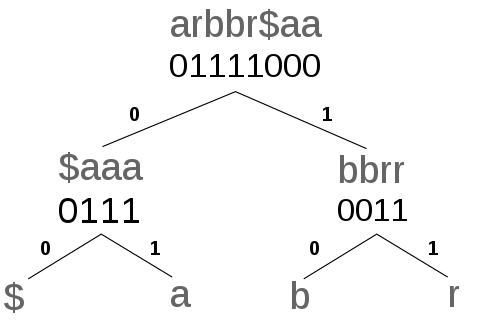
\includegraphics[width=5cm]{pictures/barbara-wavlet2.png}
\caption{Wavelet tree for "barbara" string }
\label{Wavlet-barbara}
\end{figure}

The Waveket Tree construction is done by first building 
up the left subtree by taking all the 0-encoded symbols 
${\$,a}$ and then divide them to new subtrees by re-encoding 
alphabet ${0,1,1,1}$. Notice on the first level an 'a' is 
encoded as a 0, but it is encoded as a 1 on the second 
level and at the leaf node.\\
The time complexity of Wavelet Tree for finding the number
of occurrences of a character up to specific position (rank 
query) is $\mathcal{O}\log{}\mid\sum\mid)$.\\
A rank query can be done on  $\mathcal{O}\log{}\mid\sum\mid)$ time 
as is explained in the following.
After constructing the Wavelet tree (see Figure 12), an 
rank query on the Wavelet Tree can be done on it. 
\\
In order to calculate \emph{rank(7, b)} we use the following 
procedure (illustration by Figure \ref{rank1}.\\
We know that \emph{enc(b)= 1} at the root level by 
constructing wavelet tree for the alphabet of "barbara\$"
string.

\begin{enumerate}

    \item
		 Count the number of 1s in the range[1..7], at the root node, 
		 given by \emph{rank(7,1)= 4 }. This is the index for query in 
		 0-child. 
		 
    \item
		As 'b' is encoded as 0 at the second level, calculating \emph
		{rank(4,0)= 2}. 

    \item
		Since we are at the leaf node the result of \emph{rank(7,b)} is
		equal to 2.
\end{enumerate}

\begin{figure}[H]
\centering
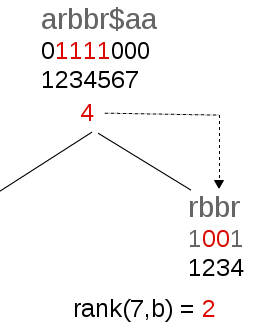
\includegraphics[width=3.75cm]{pictures/rank74.png}
\caption{The rank(7,a) over Wavelet tree for "Rhabarberbarbara" string }
\label{rank1}
\end{figure}

The space usage given Wavelet Tree structure, bits proportional to the 
depth of  Wavelet tree are needed to encode each character giving memory 
usage proportional to $\mathcal{O}(H_{0}+1)$ (Huffman coding).\\

We define \emph{$rank(n,0)= n- rank(n,1)$} and implement 
\emph{$rank(n,1)$} using the Rank9 structure \cite{rank9} 
described in Section \ref{The rank9 Data Structure}.


%%%%%%%%%%%%%%%%%%%%%%%%%%%%%%%%%%%%%%%%%%%%%%%%%%%%%%%%%%%%%%%%%%%%%%%%%%%%%%%

\subsubsection{The rank9 Data Structure} 
\label{The rank9 Data Structure}

%In this part, the layout of our data structure will be introduced.\\	

The rank9 data structure, which was first proposed by Sebastiano
Vigna\cite{rank9}, is a particular layout of bit sequences in memory
that supports rank queries in $\mathcal{O}(1)$ time.

Consider an array of 64-bit words represented as bit array 
\emph{b}. The bit at position p is stored in bit (\emph{p} 
mod 64) of $ [p \backslash 64]$ \cite{rank9}. Let a \emph
{basic block} be a subsequence of eight words starting at 
bit position \emph{p}. To construct the rank9  we divide 
the bit string into several basic blocks and then divide 
these blocks further, into words of 64 bits. We store the 
512 bits in a \emph{basic block} and two additional words 
(as described in \cite{rank9}):

\begin{enumerate}

	\item The first word (first-level count) contains the 
	total number of 1s till that position \emph{(rank(p)}).
	
	\item The second one contains the seven 9-bit values 
	(second-level counts) \emph{rank(p + 64k)- rank(p)}, 
	for 1 $\leq$ k $\leq$ 7, each shifted left by \emph
	{9(k-1)} bits.
	
\end{enumerate}

To construct the rank9  we divide the bit string into 
several basic blocks. For each basic block boundary, 
a sum of previous ranks (first-level rank) and the 
address of stored offset values(second-level rank) 
are stored which gives us an efficient rank query 
time. \\

For each block, we store:\\\\
\centerline{$ block[i].total= rank(i*512)$}\\\\
\centerline{$ block[i].subtotal[j]= rank(i*512 + (j+1)*64)-block[i].total$}\\\\
\centerline{$ b[i*8]=raw[i*512..i*512+(k+1)*64)] $}\\\\
\centerline{$ OCC_{1}(x)=block[i].total+block[i].subtotal[j-1]+popcount(b[i*8 + j],0,k)$}



\[ where
\begin{cases}
	i=[ x \backslash 512 ]\\
	j=[(x \% 512 )\backslash 64 ]\\
	k=[ x \% 64  ]\\
\end{cases}
\]


%%%%%%%%%%%%%%%%%%%%%%%%%%%%%%%%%%%%%%%%%%%%%%%%%%%%%%%%%%%%%%%%%%%%%%%%%%%%%%%%


\subsubsection{Bi-directional Wavelet Index}
\label{Bi-directional Wavelet Index}

A common way to speed up the alignment process is to index the reference string. 
Although the original BWT is a space and time efficient indexing technique for 
pattern matching problem, it only allows  searching of a pattern in one 
direction (\emph{backward} from right to the left of a pattern). 
However, for efficient inexact pattern matching, a data structure that gives us 
the ability to search for a pattern in both directions (\emph{forward}
and \emph{backward}), 
starting from the middle part of a pattern and switching between
directions, would 
be helpful. The Bi-directional Wavelet index is a data structure that solves 
this problem.

A Bi-directional Wavelet index of string S consists of \cite{bidirectional}
the \emph{backward index} that supports backward search based on the Wavelet Tree of 
the BWT string of S and the \emph{forward index} that supports backward search
on the Wavelet tree of the BWT string of the reverse string S (i.e. forward 
search on string S) denoted as $BWT^{rev}$. The main challenge is to do a 
synchronized search on the both indexes.
To illustrate it, assume that we know the $\omega$-range $[i..j]$ in the backward 
index and $\omega^{rev}$-range [$i^{rev}$..$j^{rev}$] in the forward index 
where $\omega$ is a substring of S.
Given a character $c$ and range $[i..j]$, the backward search on the backward 
index returns $c\omega$-range (by Algorithm~\ref{backward search alg}), 
but we need to find the corresponding range in the forward index and vice versa.
The Bi-directional Wavelet index of string S=barbara\$ is 
illustrated in Table \ref{bi-dir_barbara}.

\begin{table}[h]
\parbox{.45\linewidth}{
\centering
\begin{tabular}{ccl}
%\hline
i& &$S_{SA[i]}$\\
\hline
1 & a & \$ \\
2 & r & a\$ \\
3 & b & ara\$ \\
4 & b & arbara\$ \\
5 & r & bara\$ \\
6 & \$ & barbara\$ \\
7 & a & ra\$ \\
8 & a & rbara\$ 
\end{tabular}
%\caption{Foo}
}
\hfill
\parbox{.45\linewidth}{
\centering
\begin{tabular}{ccl}
%\hline
i&&$S^{rev}_{SA^{rev}[i]}$\\
\hline
1 & b & \$ \\
2 & r & ab\$ \\
3 & r & abrab\$ \\
4 & \$ & arabrab\$ \\
5 & a & b\$ \\
6 & a & brab\$ \\
7 & b & rab\$ \\
8 & a & rabrab\$ 
\end{tabular}
}
\caption{Bi-directional Wavelet index of "barbara\$".}
\label{bi-dir_barbara}

\end{table}


The range of the substring   
$\omega$ = a = $\omega^{rev}$ in both indexes is $[2..4]$.
The $ba$-range is given by $\mbox{backwardSearch}(a,[2..4])=[5\ldots 6]$
in the backward index and we want to find the $ab$-range in
the forward index.But the only information we have is that 
the suffixes of $S^{rev}$ are lexicographically ordered. \\\\
In other words \cite{bidirectional}\\\\
$S^{rev}[SA^{rev}[k]+|\omega|] < c$ for all k in $i^{rev}  \leq k  < p$,\\
$S^{rev}[SA^{rev}[k]+|\omega|] = c$ for all k in  $p  \leq  k  \leq  q $,\\
$S^{rev}[SA^{rev}[k]+|\omega|] > c$ for all k in  $q <   k \leq   j^{rev}$.\\\\
In our example of Table \ref{bi-dir_barbara},\\\\
$S^{rev}[SA^{rev}[k]+1] < b $ for no  k in $ 2 \leq k  < 5 $,\\
$S^{rev}[SA^{rev}[k]+1] = b $ for all k in $ 2  \leq  k  \leq  3 $,\\
$S^{rev}[SA^{rev}[k]+1] = r > b $ for all k in $ 3   < k  \leq  4 $.\\\\
In order to obtain this information, we need the number of smaller
and greater of all occurrence of characters in $S^{BWT}[i..j]$ 
that follow c in $\Sigma$. The Algorithm \ref{smaller-greater} 
shows  the Pseudo-code for calculating the number of all occurrences 
of characters from the alphabet $\Sigma[l..r]$ in $BWT[i..j]$ that 
are greater (smaller) than character c. In our example 
we seek to calculate the number of smaller and greater 
characters in the range of $[2..4]$ for character b.  
Following the Algorithm \ref{smaller-greater} \cite{bidirectional} 
and referring to Figure \ref{Wavlet-barbara}, character
b is encoded as 1 in the bit string of the root node (character b belongs 
to the second half $\Sigma[3..4]$ of lexicographically ordered 
alphabet $\Sigma$).
Finding the number of occurrences of characters 
in the interval [2..4] that belong to $\Sigma[1..2]$, knowing that 
they belong to the left child of the root node, we calculate\\
$$(a_{0}, b_{0})=(rank_{0} ( B^{[1..4]} ,  2-1), rank_{0} (B^{[1..4]} , 4)) = (1 , 1) $$
Moving to the right child, we compute
$$(a_{1}, b_{1})=(rank_{1} ( B^{[1..4]} ,  2-1), rank_{1} (B^{[1..4]} , 4)) = (0 , 3) $$
Since  $m=\lfloor \dfrac  {1+4}{2} \rfloor$= 2 and $b > \Sigma[2]$,
the new boundaries for next step is in the range of $[a_{1}+1..b_{1}]
=[1,3]$ and for the alphabet range of $[m+1 . . r] = [3..4]$
Proceeding recursively, we compute
$$({a}'_0, b'_{0})=(rank_{0} ( B^{[3..4]} ,  1-1), rank_{0} (B^{[3..4]}, 3)) = (0 , 2) $$
$$(a'_1, b'_{1})=(rank_{1} ( B^{[3..4]} ,  1-1), rank_{1} (B^{[3..4]}, 3)) = (0 , 1) $$
and find out that there are $b'_{1}-a'_{1}=1$ occurrences 
of character r that is greater than b and $b'_{0}-a'_{0}=2 $ 
characters that are the equal to character b.
\begin{algorithm}[H]
   \caption{}
    \begin{algorithmic}[1] 
      \Function{getBounds}{$[i..j],[l..r],c $}
        	\If{$ l = r $}
            	\State $remove last letter from Pattern$
            	\State \textbf{return} $(0,0)$
            \Else
        	     \State $(a_{0}, b_{0}) \leftarrow  rank_{0}( B^{[l..r]}, i-1), rank_{0}(B^{[l..r],j}))$
        		 \State $(a_{1}, b_{1})$ $\leftarrow$ $(i-1-a_{0}, j - b_{0}) $
        		 \State $/* (a_{1}, b_{1}) \leftarrow  rank_{1}( B^{[l..r]}, i-1), rank_{1}(B^{[l..r],j})) */$
        		 \State $m = \lfloor \dfrac  {l+r}{2} \rfloor$
        		 \If{$c \leq \sum[m]$}
        		 	\State $(smaller, greater) \leftarrow getBounds ([a_{0}+1..b_{0}],[l..m],c)$
        		 	\State \textbf{return} $(smaller, greater+b_{1}-a_{1})$
     	  		\Else 
     	  			\State $(smaller, greater) \leftarrow getBounds ([a_{1}+1..b_{1}],[m+1..r],c)$ 
     	  			\State \textbf{return} $(smaller + b_{0}-a_{0}, greater)$
     		   \EndIf
     	   \EndIf
     
    \EndFunction

	\end{algorithmic}
  \label{smaller-greater}	
\end{algorithm}

In the case of genome as a reference string, the algorithm also works if 
having BWT of the reverse complement S instead of BWT of the reverse string 
and look for the complement of pattern P.

R-Candy does not use Bi-directional Wavelet tree as its index structure 
but it has all the requirements.

It has reference genome and reverse complement of the genome and in order 
to support Bi-directional Wavelet tree just need to concatenate the two 
genome strings and search for the pattern P in both strands of the extended genome.


%%%%%%%%%%%%%%%%%%%%%%%%%%%%%%%%%%%%%%%%%%%%%%%%%%%%%%%%%%%%%%%%%%%%%%%%%%%%%%%


\subsection{R-Candy's Index Structure} 
\label{R-Candy's Index Structure}

Aligning billions of short reads to the human genome of size about 3,200 Mbps, 
calls for an efficient algorithm with optimal query time and memory space.\\ 
Since indexing the reference genome would speed up the alignment process, 
R-Candy uses a robust index structure called Wavelet Tree based FM-Index to 
lessen the time and memory complexity of its alignment process.

An overview of R-Candy's data structure is presented in Figure \ref{DSOverview}
\cite{Wavthesis}. The whole algorithm of R-Candy is a backward search on the 
BWT of the reference string. Specifically, R-Candy indexes the concatenation of
the complement of the reference genome with the reverse of the reference genome. 
The backward search uses the LF-mapping of BWT which requires a prefix-sum table
and an occurence table. The prefix-sum table could easily be calculated and saved 
in memory, but counting a given character in a prefix of the reference string
is time-consuming. Therefore to accelerate this process, strings are reduced to 
bitstrings using a  Wavelet Tree. The bit strings, with a maximum length of 
$\approx$ 6~billion, are stored in memory by the Rank9 data structure as blocks 
of $10 \times 64$-bit words, which makes the OCC table calculation very fast 
($\mathcal{O}(1)$). And subsample of the Suffix Array is used to recover the 
position of patterns in the reference genome.


\begin{figure}[H]
\centering
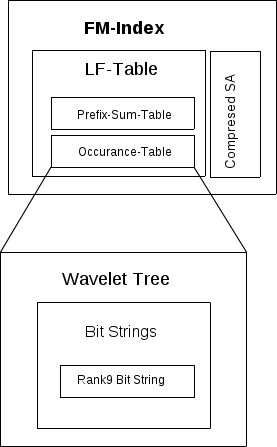
\includegraphics[width=4.75cm]{pictures/DSOverview2.png}
\caption{Overview of R-Candy's data structure }
\label{DSOverview}
\end{figure}



%%%%%%%%%%%%%%%%%%%%%%%%%%%%%%%%%%%%%%%%%%%%%%%%%%%%%%%%%%%%%%%%%%%%%%%%%%%%%%%%


\section{Method} \label{Method}

To test the performance of the R-Candy aligner for ancient DNA I developed a 
genome and NGS read simulation program, named readSim to evaluate the performance 
of R-Candy in different scenarios.

R-Candy was run on simulated reads originating from both a simulated genome and 
the human reference genome.
 

%%%%%%%%%%%%%%%%%%%%%%%%%%%%%%%%%%%%%%%%%%%%%%%%%%%%%%%%%%%%%%%%%%%%%%%%%%%%%%%

\subsection{Genome Simulation} 
\label{ Genome Simulation }


In order to make the software evaluation more informative, we decided to first 
test the aligner with a simulated genome where we have a clear expectation and
 knowledge of the true alignment of reads.

I used a probabilistic model called \emph{\nth{1} Order Markov Chain} model 
\footnote{In \nth{1} order refers to the property that the expected probabilities 
to /be/ in any state depend on one previously emitted character.} to simulate 
a genome by generating stretch of nucleotides (A, C, G, T bases) in a way that  
keeps the base composition and the CpG content of the reference genome.

A Markov chain can be drawn as a collection of states, each corresponds to a 
particular nucleotide (A, C, G, T) with arrows between them like the following 
(Figure \ref{MC}). 

Having a set of states,  $ S= \{ A, C,  G, T \}$  and probability parameter 
associated with arrows in the figure which determines the probability of 
transferring from one state to the next state (transition) and what characters 
to generate (emission).

\begin{figure}[H]
 \begin{center}
	  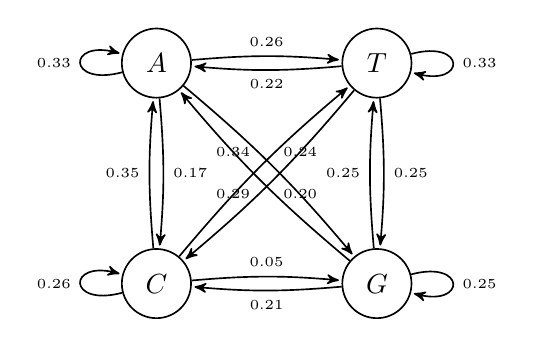
\begin{tikzpicture}[->,>=stealth',shorten >=1pt,auto,node distance=2.8cm,
                    semithick,bend angle=5]
   \tikzstyle{every state}=[fill=white,draw=black,text=black]

   \node[state]         (A)              {$A$};
   \node[state]         (T) [right of=A] {$T$};
   \node[state]         (C) [below of=A] {$C$};
   \node[state]         (G) [below of=T] {$G$};
  
   \path (A) edge [bend left]  node {\tiny 0.26} (T)
  			edge [loop left] node {\tiny 0.33} (A)
            edge [bend left]  node {\tiny 0.17} (C)
            edge [bend left]  node {\tiny 0.24} (G)
        (T) edge [loop right] node {\tiny 0.33} (T)
            edge [bend left]  node {\tiny 0.22} (A)
            edge [bend left]  node {\tiny 0.20} (C)
            edge [bend left]  node {\tiny 0.25} (G)
        (C) edge [bend left]  node {\tiny 0.34} (T)
            edge [loop left] node {\tiny 0.26} (C)
            edge [bend left]  node {\tiny 0.05} (G)
            edge [bend left]  node {\tiny 0.35} (A)
        (G) edge [loop right] node {\tiny 0.25} (G)
       	    edge [bend left]  node {\tiny 0.21} (C)
        	edge [bend left]  node {\tiny 0.29} (A)
            edge [bend left]  node {\tiny 0.25} (T);
  \end{tikzpicture}
  \caption{Trained \nth{1} order Markov chain based on human reference genome}
  \label{MC}
 \end{center}
\end{figure}


As mentioned above, these probabilities are called \emph{transition}, which are 
calculated by counting the number of state given its previous state ($ A \rightarrow 
A, A\rightarrow C, A \rightarrow T, A \rightarrow G, C \rightarrow C,$ ...) in 
the genome of interest; see the Table \ref{transition-table} (Filled with human 
reference genome bases consistency). And then create a \emph{Transition Matrix} 
by calculating the frequency of seeing each transition, as is shown in Figure 
\ref{transition-matrix}.\\

\begin{table}[h]
  \begin{tabular}{ |  p{1cm} | p{2cm} | p{2cm} | p{2cm} | p{2cm} |}
    \hline
  	%\textbf{Type} & \textbf{Read length } &\textbf{Running time(s) } 
  	%&\textbf{Speed \hspace{35pt}(no. of reads/s)} \\ \hline
  	  
 	             & A   & C & G & T \\ \hline
      A  & 279630175  & 143865843 & 199830254 & 220834783 \\ \hline
 	  C	 & 207298683  & 148996334 & 28155478 & 199938031\\ \hline
 	  G	 & 169559114  & 121898050 & 149073778 & 144192413\\ \hline
 	  T  & 187672847  & 169629108  & 207663790 & 280419080\\ \hline
      
 	  
   \end{tabular}
%\caption{Transition number for a genome sequence of length 
%1G bp and chromosomes of length 250M bp.}
  \caption{Transition probabilities for human reference genome}
 \label{transition-table}
\end{table}

%And then calculate the frequency of seeing each transition 
%called \emph{Transition Matrix}, as shown below.


\begin{figure}[H]
 \centering
\[
T = 
 \begin{pmatrix}
   &  A  & C & G & T  \\
 A & 0.331252 & 0.170425 & 0.236721 & 0.261603  \\
 C & 0.354727 & 0.254961 & 0.0481794 & 0.342132  \\
 G & 0.289982 & 0.208471 & 0.254948 & 0.246599  \\
 T & 0.221997 & 0.200653 & 0.245644 & 0.331706 \\
  
 \end{pmatrix}
\]
 \caption{Transition Matrix for human reference genome}
 \label{transition-matrix}
\end{figure}


A starting position (S) is weighted by steady state probabilities
and no specific probability for an end state(E) is defined. 
Because the generated sequence can end with any character, 
in other words, the \emph{Markov} model can terminate in any state. 
(Figure \ref{MC_SE}).

\begin{figure}[H]
 \begin{center}
 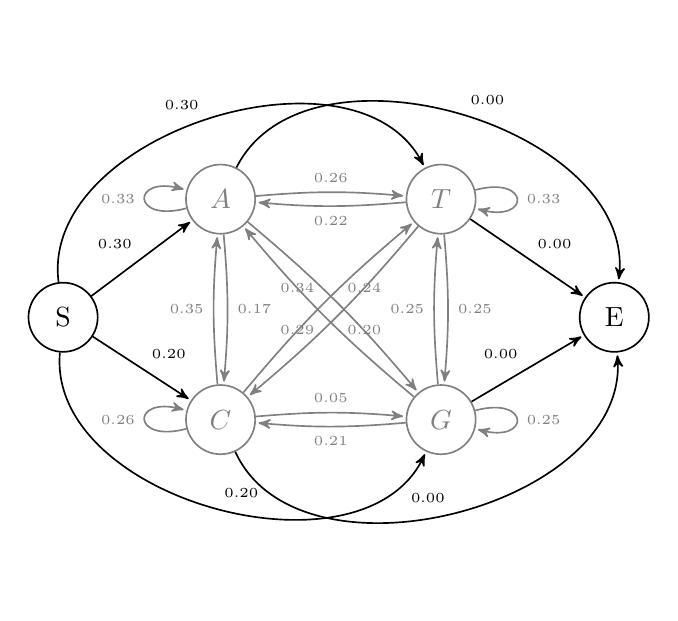
\begin{tikzpicture}[->,>=stealth',shorten >=1pt,auto,node distance=2.8cm,
                    semithick,bend angle=5]
  \tikzstyle{every state}=[fill=white,draw=gray,text=gray]

  \node[state]         (A)              {$A$};
  \node[state]         (T) [right of=A] {$T$};
  \node[state]         (C) [below of=A] {$C$};
  \node[state]         (G) [below of=T] {$G$};
  \node[state]         (S) [draw=black, text= black]at (-2,-1.5) {S};
  \node[state]         (E) [draw=black, text = black]at (5 ,-1.5) {E};
  
  \path (A) edge [gray, bend left]  node {\tiny 0.26} (T)
  			edge [gray, loop left] node {\tiny 0.33} (A)
            edge [gray, bend left]  node {\tiny 0.17} (C)
            edge [gray, bend left]  node {\tiny 0.24} (G)
            edge [bend left=80]  node {\tiny 0.00} (E)
        (T) edge [gray, loop right] node {\tiny 0.33} (T)
            edge [gray, bend left]  node {\tiny 0.22} (A)
            edge [gray, bend left]  node {\tiny 0.20} (C)
            edge [gray, bend left]  node {\tiny 0.25} (G)
            edge   			  node {\tiny 0.00} (E)
        (C) edge [gray, bend left]  node {\tiny 0.34} (T)
            edge [gray, loop left] node {\tiny 0.26} (C)
            edge [gray, bend left]  node {\tiny 0.05} (G)
            edge [gray, bend left]  node {\tiny 0.35} (A)
            edge [bend right=80]  node {\tiny 0.00} (E)
        (G) edge [gray, loop right] node {\tiny 0.25} (G)
       	    edge [gray, bend left]  node {\tiny 0.21} (C)
        	edge [gray, bend left]  node {\tiny 0.29} (A)
            edge [gray, bend left]  node {\tiny 0.25} (T)
            edge   			  node {\tiny 0.00} (E)
        (S) edge   			  node {\tiny 0.30} (A)
       	    edge   			  node {\tiny 0.20} (C)
        	edge [bend right=80]  node {\tiny 0.20} (G)
            edge [bend left=80]  node {\tiny 0.30} (T)
       
            ;
;
 \end{tikzpicture}
 \caption{Trained \nth{1} Order Markov-Chain based on the human reference
  genome with start and end states}
 \label{MC_SE}
 \end{center}
\end{figure}

The simulation program asks for the length of the genome and then the Markov chain 
model starts at one of the states weighted by the steady state probabilities and 
continuously walks between states based on their probabilities on transition matrix 
till the number of visited states is reached, given the genome length. 


%%%%%%%%%%%%%%%%%%%%%%%%%%%%%%%%%%%%%%%%%%%%%%%%%%%%%%%%%%%%%%%%%%%%%%%%%%%%%%%


\subsection{Read Simulation} \label{Read Simulation}

Simulated reads that capture different characteristics of DNA reads are the 
second part of my test data in this evaluation.

Three types of reads simulating different properties of a genome used in this
 evaluation are

\begin{itemize}
	\item fresh DNA reads
	\item ancient DNA reads
	\item exogenous reads
\end{itemize}

\textbf{Fresh DNA Simulation}\\

The following workflow is used by readSim to simulate fresh DNA
 reads:

\begin{enumerate}
 \item Uniformly sample reads of length 25-40 bps from the reference genome.

 \item Introduce a given number of differences to 
 reads in order to simulate different divergence rates
 (see Section \ref{Divergence}).

 \item Add the specific types of errors introduced by the sequencing 
 machine based on empirical cumulative distribution or ART\cite{art} 
 (see Section \ref{Sequencing Error and Base Quality Score}).
\end{enumerate}


\textbf{Ancient DNA Simulation} \\

The workflow for simulating ancient DNA reads follows the workflow used for 
simulating fresh DNA reads with one extra step

\begin{itemize}
 
\item Simulate \emph{post-mortem} deamination damage based on 
deamination parameters (i.e. overhang and non-overhang deamination 
rate in addition to the probability of being in overhang) by users
(see Section \ref{Deamination}). 

\end{itemize}

as third step in the workflow and sequencing error will be
the fourth in simulation ancient DNA reads.\\

\textbf{Simulation of exogenous Reads }\\

Ancient DNA extracts are often highly contaminated by mostly environmental 
microbes that always make the recognition of endogenous and exogenous DNA 
hard. Although there is a database of known exogenous DNAs that could help 
us to detect exogenous sequences and don't mix them with endogenous DNA 
sequences, there are still a lot of unknown contaminants.
\\\\
In order to have a realistic simulation of the exogenous DNA present in ancient
samples, we decided to simulate exogenous DNA sequences, in addition to, our 
genomic DNA read simulations.
\\\\
The exogenous read simulation workflow is the following 

\begin{enumerate}

 \item Generate a random string of DNA nucleotides (A, C, G, T) 
 for a given length (Chance of seeing each nucleotide is the same as any
  other one and equal to 0.25).

\item Simulate \emph{post-mortem} deamination damage based on deamination
 parameters (i.e. overhang and non-overhang deamination rate in addition to 
 the probability of being in overhang) specified by the user. 

 \item Add the specific types of errors coming from sequencing machine 
 based on empirical cumulative distribution or ART\cite{art} .

\end{enumerate}




%%%%%%%%%%%%%%%%%%%%%%%%%%%%%%%%%%%%%%%%%%%%%%%%%%%%%%%%%%%%%%%%%%%

\subsubsection{Divergence} \label{Divergence}

By definition \emph{\quotes{divergence is the separation
of a population's gene pool from the gene pools of other populations 
due to mutation, genetic drift, and selection\cite{divergence1}.}}

For biological reasons, we expect some divergence between
the aligned reads and reference genome when aligning an individual 
to the genome of a closely related species.

To test the performance, different divergence rates are simulated by 
a fixed number of mismatches per read. Therefore, an expected performance 
number for any real world situation with a certain substitution rate due to 
divergence can be extrapolated from that.
 
 
%%%%%%%%%%%%%%%%%%%%%%%%%%%%%%%%%%%%%%%%%%%%%%%%%%%%%%%%%%%%%%%%%%%%%%%%%%%%%%%%%%%%%%%%%%%%%% 

\subsubsection{Sequencing Error and Base Quality Score} 
\label{Sequencing Error and Base Quality Score}
 

A quality score indicating the confidence level of correctly seeing a 
base is assigned to each base of a read sequence, in other words, it 
demonstrates the probability that a base is called incorrectly by a 
sequencing machine and is encoded in logarithmic states for practical 
reasons.

Phred quality score (Q score) is the most widely used metric
indicating quality score.


Phred quality scores are defined as \cite{phred2}:

$$ Q = -10  log_{10}P   $$
$$  or $$
$$ P = 10 ^ { \frac{-Q}{ 10 } } $$


A typical base quality score of Illumina platform for the majority of 
bases is Q30 and above which provides an ideal level of accuracy for a 
range of sequencing applications. 
A quality score of 30 (Q30) predicts one base call in 1000 be incorrect
and corresponds to call accuracy of 99.9\%.

A sequencing error is an incorrect identification of a nucleotide base 
resulting from an inaccurate machine read. Due to an unavoidable error 
in the base calling, generally, there is no precise DNA sequencing. 

Sequencing error rates are higher than divergence and deamination
on this model sequence and are not uniformly distributed. They tend to 
cluster at the end of the reads lead to a lower quality score rate at 
the end of the reads.

Different sequencing platform has different quality scores indicating 
variable sequencing error. These errors become visible when aligning a 
read to a reference string as substitutions or mismatches.

The main sequencing error for Illumina platform is base substitution 
\cite{art}. The substitution error probability is calculated by the 
base quality score along with the called base.

The output data of sequencing machines significantly differs in quality for 
several reasons (for illustration, see Ewing et al. 1998).  Therefore, an 
effective measure for the reliability of such a data is vital\cite{phred1}.\\


In order to implement sequencing error for simulated reads, There are two
options in my simulator (readSim):

The \textbf{first} option uses a next-generation sequencing read simulator 
(ART) to produce base quality and simulate sequencing error.


The \textbf{second} option for simulating sequencing error which is used for
my evaluation in this thesis is based on an empirical sequencing error profile 
data (in-house sequenced data).

The implementation looks at the quality values assigned to each base at each
position in the read and generates a distribution table for it (figure \ref{hist}).

\begin{figure}[H]
\centering
%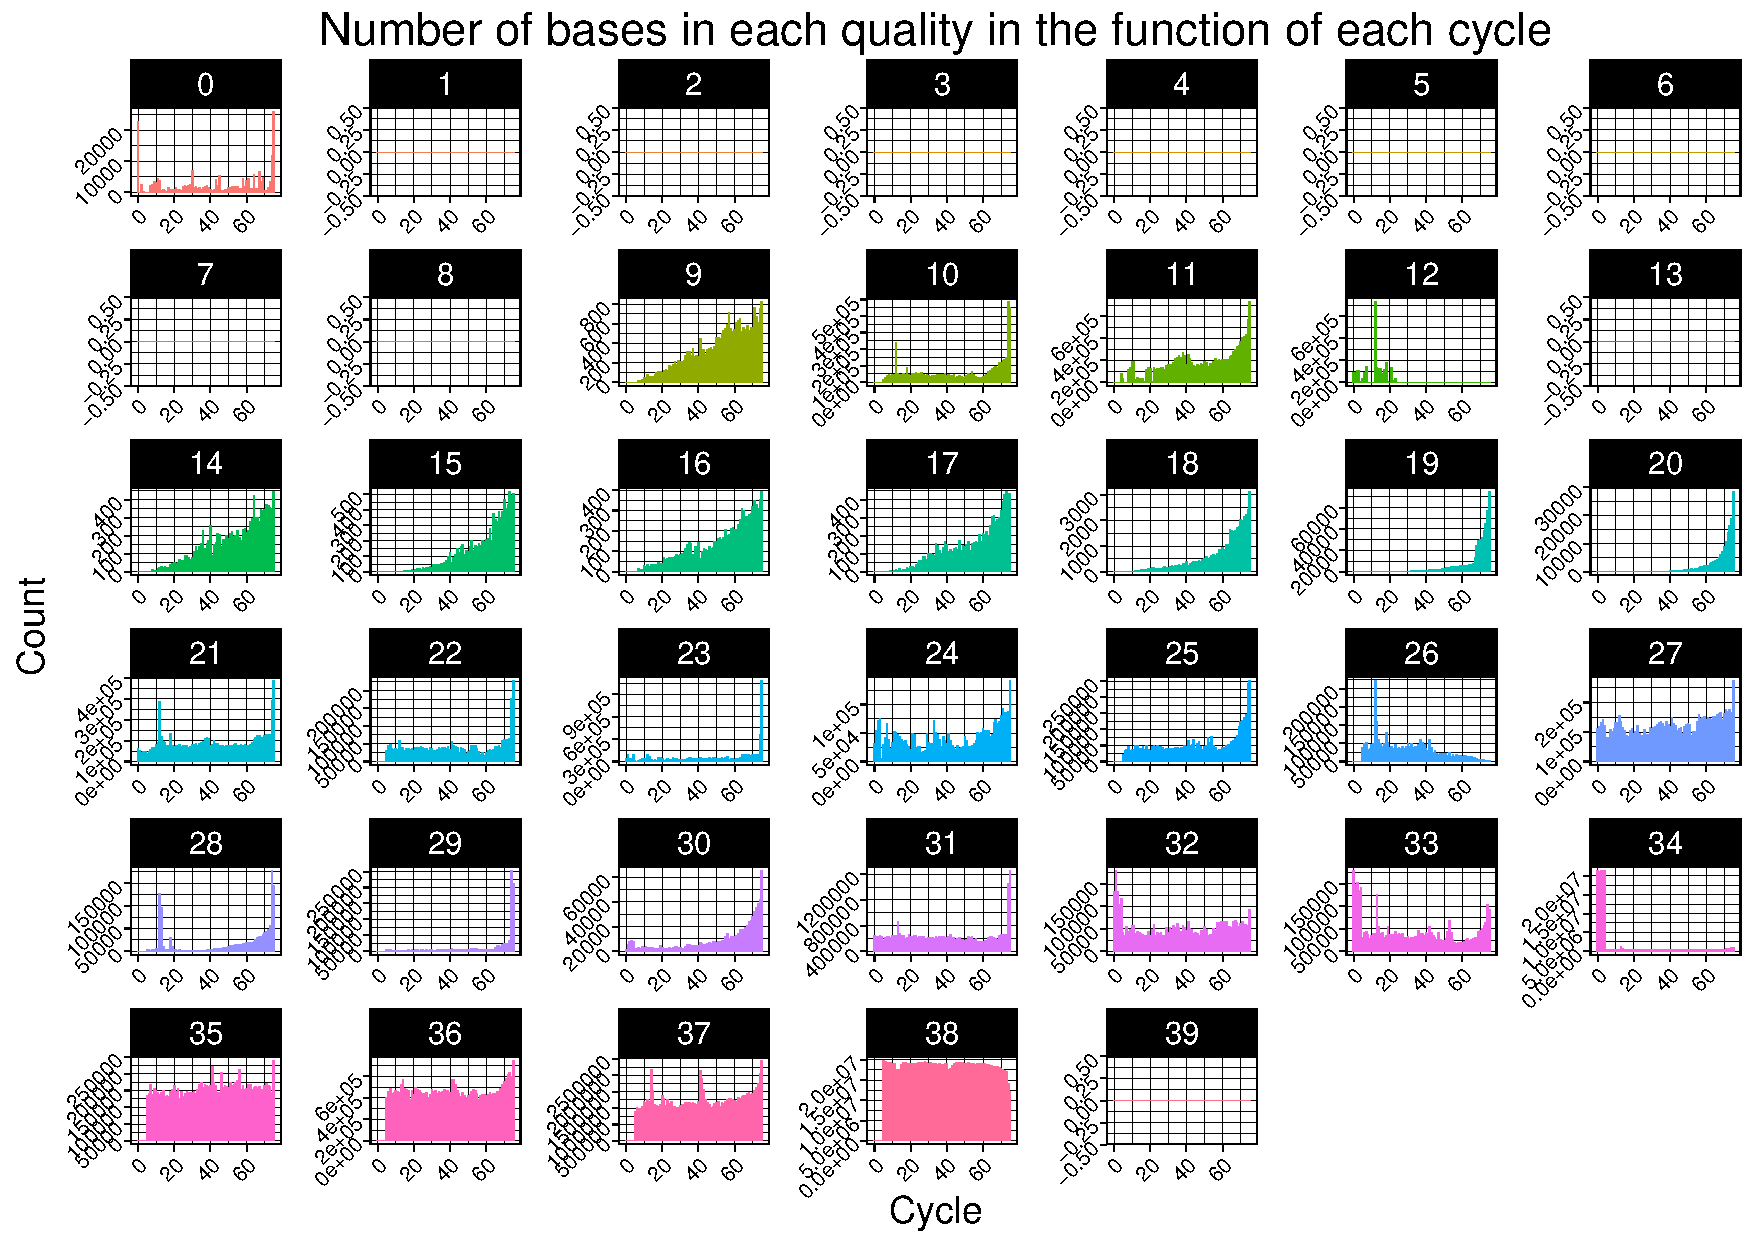
\includegraphics[width=12cm]{pictures/Rplot_quality.pdf}
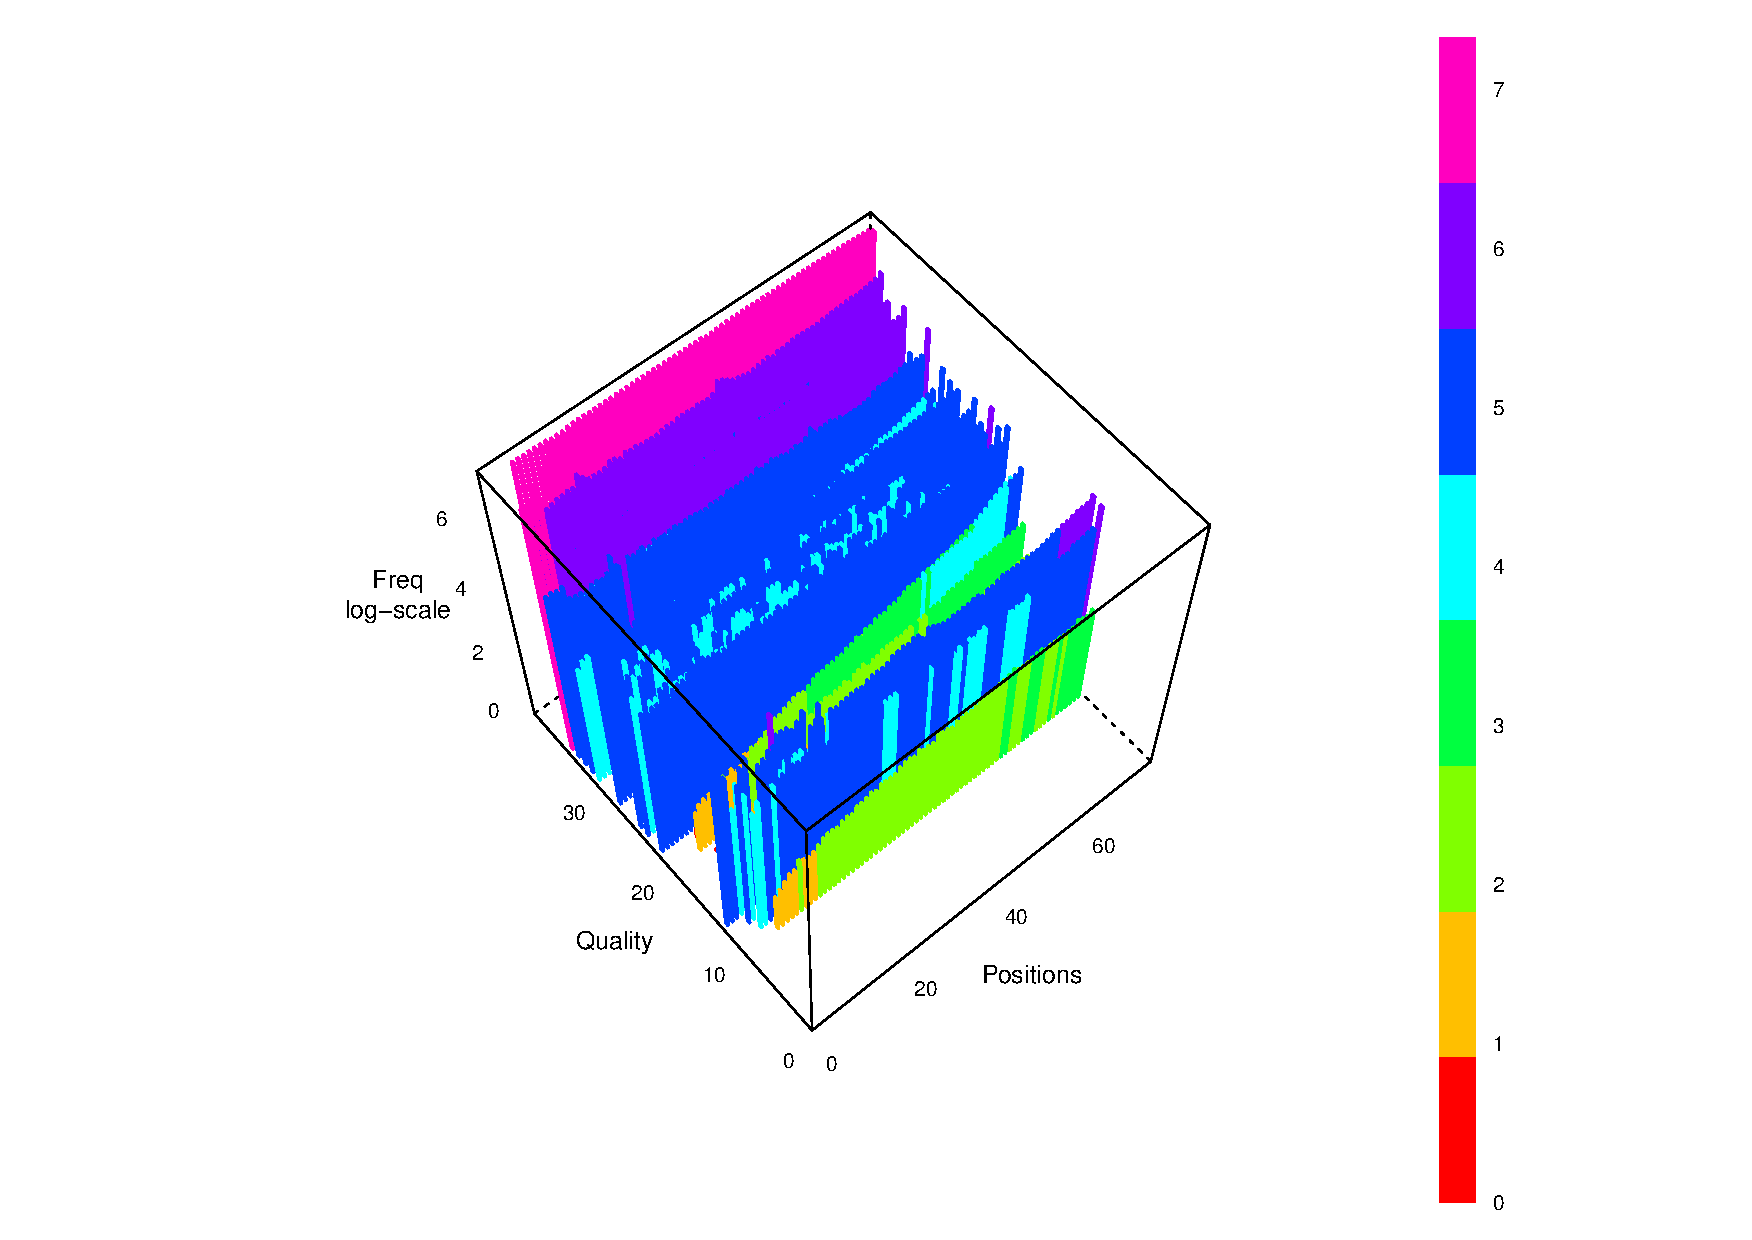
\includegraphics[width=12cm]{pictures/3Dplot.pdf}
\caption{Number of bases in each cycle as a function of having certain quality}
\label{hist}
\end{figure}

It then calculates the probability mass function (PMF) which is the quality 
frequencies at each cycle for both forward and reverse reads. At the next 
step, cumulative distribution function (CDF) is calculated by summing up the 
quality frequency of each base with all quality bases before it (Figure \ref{CDF}).

\begin{figure}[H]
\centering
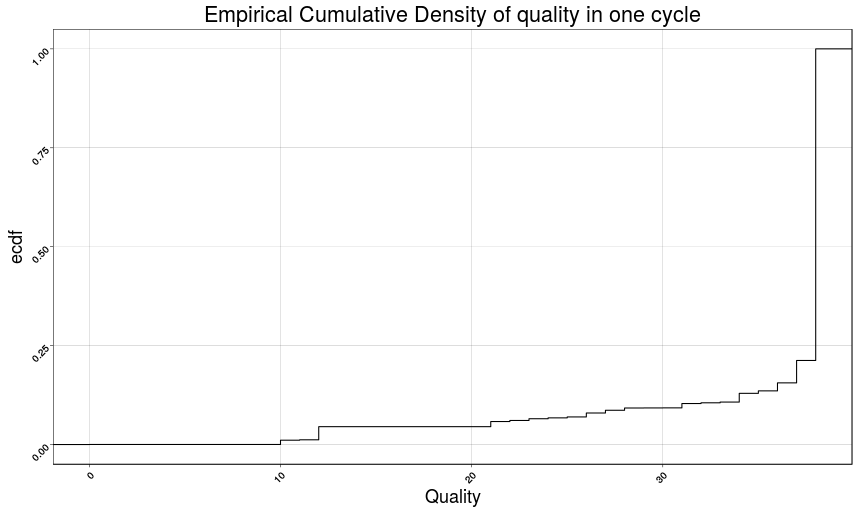
\includegraphics[width=12cm]{pictures/Rplot_ecdf.png}
\caption{Empirical cumulative distribution of all bases in cycle 11 of all forward 
reads}
\label{CDF}
\end{figure}

%%%%%%%%%%%%%%%%%%%%%%%%%%%%%%%%%%%%%%%%%%%%%%%%%%%%%%%%%%%%%%%%%%%%%%%%%%%%%%%%%%

\subsubsection{Deamination} \label{Deamination}

A high nucleotide misincorporation rate of thymine(T) in place o
cytosine(C) is the unique characteristic of ancient DNA as the result of
\emph{post-mortem} DNA damage.  This is thought to occur, because
cytosine spontaneously converts to uracil, which is sequenced as
thymine(T), through hydrolytic deamination
\cite{mapdamage2}\cite{damagepattern}.

In order to simulate the effect of deamination on aDNA, 
Philip Johnson's deamination model\cite{mapdamage2}  
with small tweaks for single-stranded reads is used.

For single stranded library preparation,
let $\sigma$ and $\sigma'$ be deamination rate in the 5' 
and 3' overhangs respectively assuming different deamination rate 
in the two overhang and $\lambda$ be the overhang length. 
Let  $\delta$ be the deamination rate in non-overhang parts 
where $l$ is the read length.


The DNA damage transition matrix is defined as:

$$ P_{dam} = 
 \begin{pmatrix}
  1 & 0 & 0 & 0 \\
  0 & 1-p_{ct} & 0 & p_{ct} \\
  0  & 0  & 1 & 0  \\
  0 & 0 & 0 & 1 
 \end{pmatrix}$$
 
Where columns and rows representing substitution rate between 
bases in the reference sequence and a read respectively.\\
The probability of damage for each base is defined as 

\[ P_{ct}(i, \sigma, \sigma', \delta, l, \lambda ) 
\begin{cases}
    \sigma  \quad if \quad i < \lambda  \\
    \sigma' \quad if \quad i \geq l-\lambda \\
    \delta \quad otherwise  \\
\end{cases}
\]

The probability of being in overhang is provided by the user as the 
\emph{success fraction} value $P$ in the geometric cumulative distribution 
function (CDF). Also for the simplicity, we assume the damage probability 
of each base  in an overhang is independent of the other bases. In other 
words, deaminating of one base has no influence on the other bases.\\

$$Pr( \lambda = k ) = 1 - (1 - p)^{k}$$
$$ k = 1, 2, 3, ... $$

In the simulation, half of the reads have highly deaminated overhangs
with geometrically distributed lengths. The simulation program calculates 
the overhang length given the user-specified success fraction value.
And then the user-specified substitution ratio numbers of $ \sigma $ 
and $\sigma' $,  are used for substitution of the $ C \rightarrow T$ 
in overhangs. The deamination substitution  in non-overhang parts is 
applied with substitution ratio of $\delta$.



%%%%%%%%%%%%%%%%%%%%%%%%%%%%%%%%%%%%%%%%%%%%%%%%%%%%%%%%%%%%%%%%%%%%%%%%%%%%%%%%%


\subsection{Evaluation Criteria} \label{Evaluation Criteria}

Evaluation of R-Candy is done based on three aspects, namely, 
the mapping accuracy, the throughput and memory footprint.

\begin{itemize}

 \item The mapping accuracy: mapping accuracy is divided into two parts, 
 sensitivity (true positive rate) and specificity (false positive rate).

Reported sensitivity on simulated genome is the number of correctly mapped
(mapped to the read's original position in the reference genome) genomic reads 
divided by the total of simulated genomic reads. The one true alignment of the
reads is known due the clear structure of the genome. In the case of the real 
genome (e.g. human genome) with some repetitive elements, R-Candy's output for 
such reads will be multiple alignments. Therefore, in the case of multiple hits, 
an arbitrary alignment from the set of multiple best hits (reads with the best 
alignment score) is chosen and evaluated by checking the aligned position given 
the known true position of the read.\\

The false positive rate is defined as the number of aligned exogenous reads 
divided by the total number of exogenous reads.

 \item The aligner's throughput: the number of mapped reads per second (bps/sec).

 \item The memory footprint: the required memory by the tool for indexing the 
reference string, processing the reads and storing them. 

\end{itemize}
 


%%%%%%%%%%%%%%%%%%%%%%%%%%%%%%%%%%%%%%%%%%%%%%%%%%%%%%%%%%%%%%%%%%%%%%%%%%%%%%%% 


\section{Results and Discussion} \label{Results and Discussion}

R-Candy is an experimental alignment program for ultra short ancient DNA sequences 
(25-50 bps) based on BWT of the reference genome. It is written in Haskell. It 
performs semi-global alignment for single reads, generates an alignment score 
and reports all possible hits for each read. It is the first aligner that takes 
into account the specific characteristic of ancient DNA \emph{post-mortem} 
deamination damage.

We compared the performance of R-Candy to another aligner that uses the 
Burrows-Wheeler transform\cite{bwa} on a number of simulated data-sets modeling 
different types of reads. 

BWA is a widely used aligner for short reads including ancient DNA sequence 
reads. It has been widely used as aligner for ancient DNA by increasing the 
number of mismatches and gaps allowed. However, it includes no model of ancient 
DNA damage, and is not particularly well-suited for alignment of very short reads.



%%%%%%%%%%%%%%%%%%%%%%%%%%%%%%%%%%%%%%%%%%%%%%%%%%%%%%%%%%%%%%%%


\subsubsection*{Evaluation Scenarios} \label{Evaluation Scenarios}

A simulated genome is used for evaluation due to its simple structure 
and clear expectations and results. 

Evaluation on a real genome is used to confirm R-Candy's behavior 
on simulated genome despite the differences between the two genomes.

The accuracy of the aligners is evaluated as explained in Section
 \ref{Evaluation Criteria}.

Simulated reads extracted from both simulated and the human genome
(version hg19) are in 4 different short lengths of 25, 30, 35, and 
40 base pairs typical of ancient DNA getting aligned back to the 
reference genome by BWA and R-Candy (as is described in Table 
\ref{test-scenarios}).

The results show R-Candy's performance on a different range of 
alignment scores cutoffs from 1 to 20.



\begin{table}[ht]
\centering
\begin{adjustbox}{max width=\textwidth}
\begin{tabular}{|c|c|c|c|c|c|c|c|c|}\cline{2-9}

\multicolumn{1}{c|}{\multirow{2}{*}{}}  &\multicolumn{2}{c|}{\textbf{DNA Reads}} 
&\multicolumn{2}{c|}{\textbf{Extracted From}} &\multicolumn{2}{c|}{\textbf{Aligned To}} 
&\multicolumn{2}{c|}{\textbf{Parameters}}\\\cline{2-9}

\multicolumn{1}{c|}{} & Fresh & Ancient & Simulated & Real & Simulated & Real &  Default & Ancient \\
\multicolumn{1}{c|}{} &	& &	Genome	& Genome & Genome & Genome & (No Deamination) & \\\hline
 
\textbf{Scenario 1} & \checkmark & & \checkmark & & \checkmark & & \checkmark & \\\hline

\textbf{Scenario 2} & \checkmark & &  & \checkmark &  & \checkmark & \checkmark & \\\hline

\textbf{Scenario 3} & \checkmark  & & \checkmark & & \checkmark & &  & \checkmark \\\hline

\textbf{Scenario 4} & \checkmark & &  & \checkmark &  & \checkmark &  & \checkmark \\\hline

\textbf{Scenario 5} &  & \checkmark &\checkmark  &  &\checkmark &  & &  \checkmark \\\hline

\textbf{Scenario 6} &  & \checkmark & & \checkmark & & \checkmark & &  \checkmark \\\hline

\end{tabular}
\end{adjustbox}
\end{table}


%%%%%%%%%%%%%%%%%%%%%%%%%%%%%%%%%%%%%%%%%%%%%%%%%%%%%%%%%%%%%%%%%%%%%%%%%%%%%%%%


\subsection{Evaluation on Simulated Fresh DNA Reads } 
\label{Simulated Fresh DNA Reads }
 
The purpose of these tests is to see the performance of R-Candy on fresh DNA 
sequences aligning R-Candy's default parameters. 



%%%%%%%%%%%%%%%%%%%%%%%%%%%%%%%%%%%%%%%%%%%%%%%%%%%%%%%%%%%%%%%%%%%%%%%%%%%%%%%%


\subsubsection {Alignment of Simulated Fresh DNA Reads to a Simulated Genome 
with default parameters.}

\label {Alignment of Simulated Fresh DNA Reads to a Simulated Genome with 
default parameters.}
 
 
 \begin{itemize}

   \item \textbf{Data:} Simulated fresh DNA extracted from a simulated genome 
   with between 0 and 6 substitutions to allow increasing sequence divergence
   and including sequencing error generated from empirical quality distribution 
   data.
 
   
   \item \textbf{Reference genome:} Reads were aligned to a simulated genome of 
   length 1Gb.

    \item \textbf{Aligners:} 
     R-Candy with default parameters and alignment score cutoff of 20. \\
     BWA version 0.5.10-evan.10 with default parameters and ancient parameters 
     (the mismatch parameters set to
     0.01 and the number of gap opens to 2)\cite{green2010draft}.

  \end{itemize}
 
Here we aim to evaluate the performance of R-Candy on fresh DNA reads 
without using the deamination parameters (R-Candy's default parameters).


\begin{figure}[H]
\centering
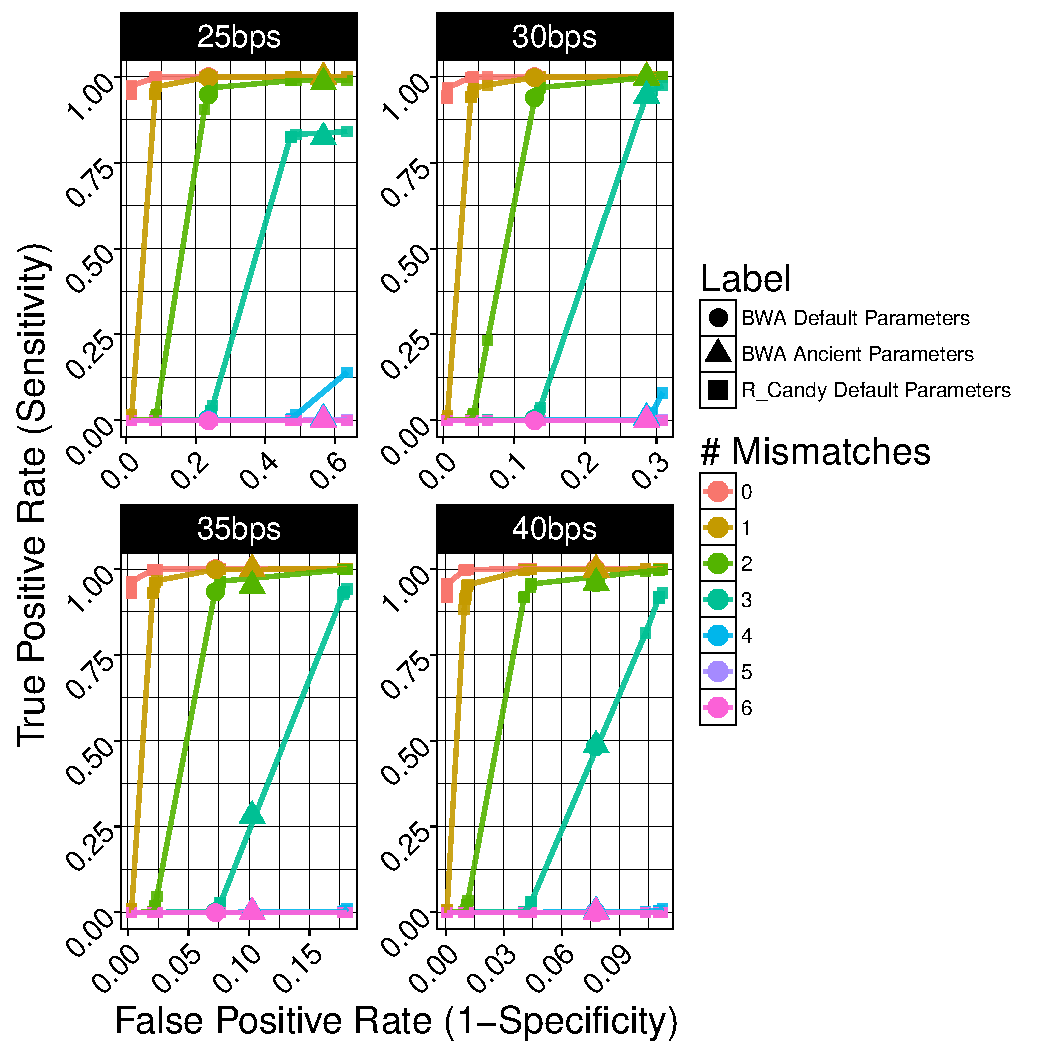
\includegraphics[width=12cm]{pictures/f_DS3_emp.pdf}
\caption{
ROC curve for the alignment to the simulated reference genome of simulated 
fresh sequence reads. See Section \ref{Evaluation Scenarios} 
for more details.}
\label{DS3_emp}
\end{figure}


As the results in Figure \ref{DS3_emp} show, when aligning fresh DNA reads with 
no damage parameters, R-Candy and BWA aligners with default parameters, perform
equally well. However, for some define AS cutoffs R-Candy shows a moderately higher 
sensitivity compared to BWA with ancient parameters.

Increasing the length of the reads improves the specificity (higher specificity 
means lower rate of spurious alignments of exogenous reads) of both BWA with 
ancient parameters and R-Candy for lower cutoff values.



%%%%%%%%%%%%%%%%%%%%%%%%%%%%%%%%%%%%%%%%%%%%%%%%%%%%%%%%%%%%%%%%%%%%%%%%%%%%%%%%


\subsubsection{ Alignment of Simulated Fresh DNA Reads to the Human Reference Genome
with default parameters.}

\label{ Alignment of Simulated Fresh DNA Reads to a the Human Reference Genome with
default parameters.}


 \begin{itemize}
 
   \item \textbf{Data:} Simulated fresh DNA extracted from a simulated genome 
   with between 0 and 6 substitutions to allow increasing sequence divergence
   and including sequencing error generated from empirical quality distribution
   data.
   
   \item \textbf{Reference genome:} Reads were aligned to the human genome 
   (version hg19) of length 3.2 Gb.

    \item \textbf{Aligners:} 
    R-Candy with default parameters and alignments score cut-off of 20. \\
    BWA version 0.5.10-evan.10 with default parameters and ancient parameters
    (the mismatch parameter set to 0.01 and the number of gap  opens to 2)
    \cite{green2010draft}.
	
 \end{itemize}
	
	
Here we aim to evaluate the performance of R-Candy on fresh DNA reads, aligned 
to the human reference genome without using the deamination parameters (R-Candy's 
default parameters).


\begin{figure}[H]
\centering
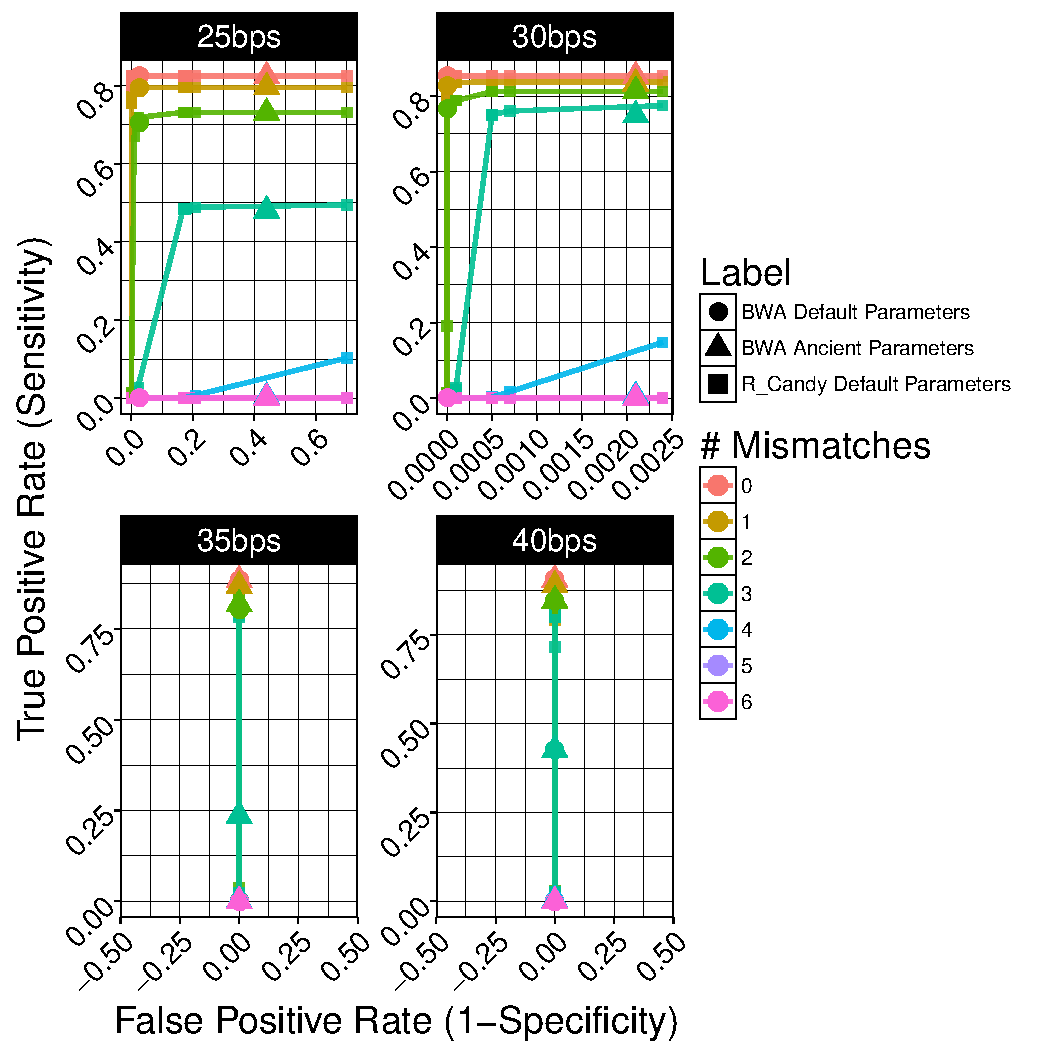
\includegraphics[width=11cm]{pictures/f_DS6_emp.pdf}
\caption{ 
ROC curve for the alignment to the human reference genome of simulated 
fresh sequence reads. See Section \ref{Evaluation Scenarios} 
for more details.
}
\label{DS6_emp}
\end{figure}
 


The result of aligning fresh DNA reads extracted from the human genome and 
aligned back to it ( Figure \ref{DS6_emp} ) confirms the result of the similar 
test on the simulated data on scenario 1.  However, it shows a lower specificity 
on the length 30 on the human genome for both BWA ancient and R-Candy compared
to the same test on the simulated genome.

Results show a big difference in specificity between length 25 bps and 30 bps, 
where increasing the length decreases the rate of spurious alignments of exogenous
reads.

The plots show no spurious alignments of contaminant exogenous reads of length 
35 bps and 40 bps, by either of the aligners.

The other observation on the plots, shows the sensitivity of the both aligners
to the divergence.


%%%%%%%%%%%%%%%%%%%%%%%%%%%%%%%%%%%%%%%%%%%%%%%%%%%%%%%%%%%%%%%%%%%%%%%%%%%%%%%%%%%%%%


 \subsubsection {Alignment of Simulated Fresh DNA Reads to a Simulated Genome 
 with ancient parameters.}

 \label {Alignment of Simulated Fresh DNA Reads to a Simulated Genome with
 ancient parameters.}
 

  \begin{itemize}

   \item \textbf{Data:} Simulated fresh DNA extracted from a simulated genome 
   with between 0 and 6 substitutions to allow increasing sequence divergence
   and including sequencing error generated from empirical quality distribution 
   data.
 
   
   \item \textbf{Reference genome:} Reads were aligned to a simulated genome of 
   length 1Gb.

    \item \textbf{Aligners:}
    R-Candy with ancient parameters (deamination damage, -l left overhang 
    parameter = 0.3, -r right overhang parameter= 0.3 , -d deamination rate 
    in double stranded section = 0.02 , -s deamination rate in single stranded 
    section = 0.9 ) and cutoff for alignment score at 20. \\
    BWA with default parameters and ancient parameters \cite{green2010draft}
    (mismatch parameter -n set to 0.01 and the number of gap openings -o to 2)
   
   \end{itemize}
 
Here we aim to evaluate the performance of R-Candy on fresh DNA reads while 
using ancient DNA parameters. This allows us to determine whether fresh DNA
can be aligned accurately using ancient parameters. 


\begin{figure}[H]
\centering
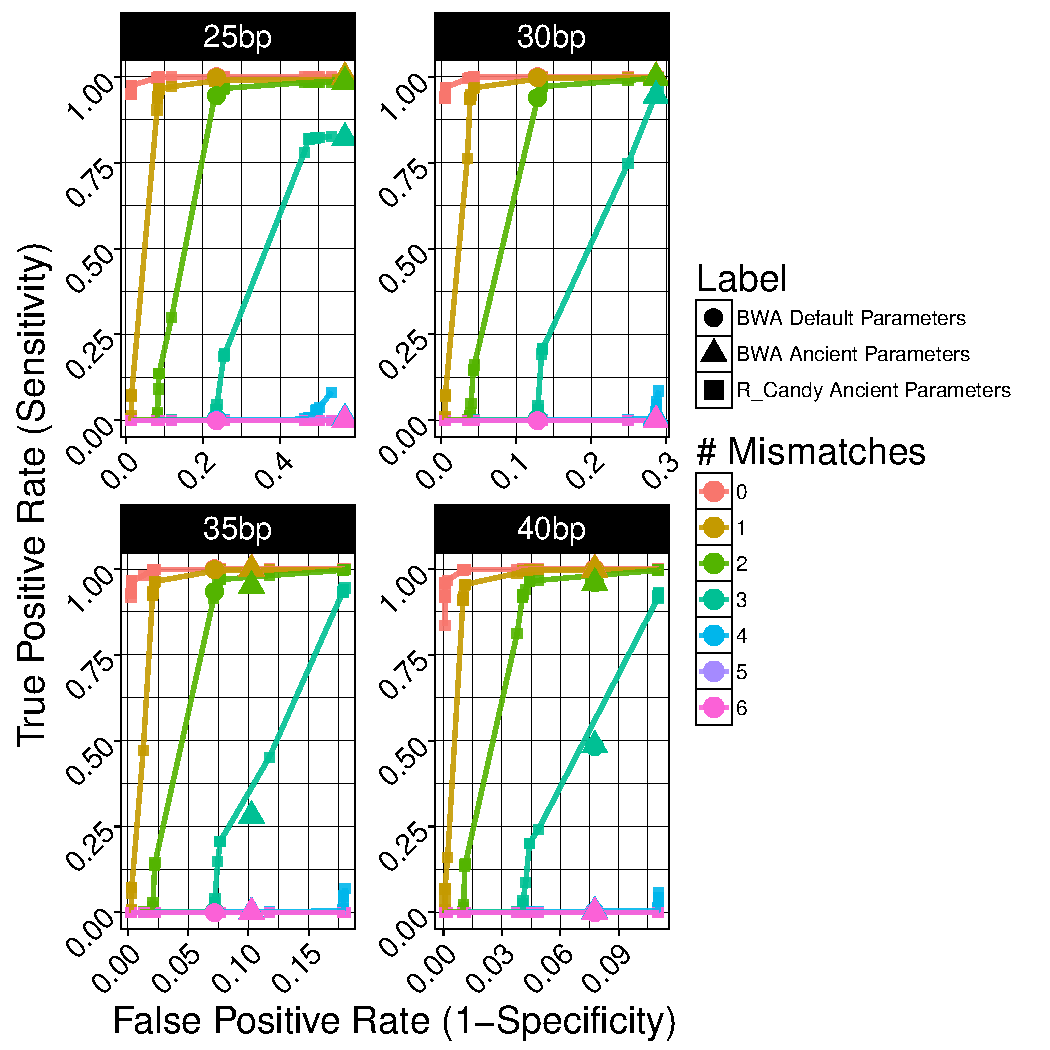
\includegraphics[width=12cm]{pictures/f_DS8_emp.pdf}
\caption{ ROC curve for the alignment to the simulated reference genome of 
simulated fresh sequence reads aligned by ancient parameters. See Section 
\ref{Evaluation Scenarios} for more details.}
\label{DS8_emp}
\end{figure}


Aligning fresh DNA reads by R-Candy with ancient parameters and BWA with default 
parameters, perform equally well, While using BWA with ancient parameters just 
increases the false positive rate as is the case for using higher AS cutoffs for 
R-Candy.

Increasing the length of the reads reduces false positive rates (specificity)  
where in the length of 40 bps we see the same behavior of BWA aligned by default
and ancient parameters.


%%%%%%%%%%%%%%%%%%%%%%%%%%%%%%%%%%%%%%%%%%%%%%%%%%%%%%%%%%%%%%%%%%%%%%%%%%%%%%


\subsubsection{ Alignment of Simulated Fresh DNA Reads to a the Human Reference Genome
with ancient parameters.}

\label{ Alignment of Simulated Fresh DNA Reads to a the Human Reference Genome.}


 \begin{itemize}
 
   \item \textbf{Data:} Simulated fresh DNA extracted from a simulated genome 
   with between 0 and 6 substitutions to allow increasing sequence divergence
   and including sequencing error generated from empirical quality distribution
   data.
   
   \item \textbf{Reference genome:} Reads were aligned to the human genome 
   (version hg19) of length 3.2 Gb.

    \item \textbf{Aligners:}
    R-Candy with ancient parameters 
  	(deamination damage, -l left overhang parameter= 0.3, -r right overhang parameter= 0.3 , 
	-d deamination rate in double stranded section = 0.02 , 
	-s deamination rate in single stranded section = 0.9 )
  	and cutoff for alignment score at 20. \\
  	BWA with default parameters and ancient parameters \cite{green2010draft}
   	(mismatch parameter -n set to 0.01 and the number of gap openings -o
   	to 2)
   
 \end{itemize}
	
	
Here we aim to evaluate the performance of R-Candy on fresh DNA reads, 
aligned to the human reference genome while using the ancient parameters
(deamination damage parameters).


\begin{figure}[H]
\centering
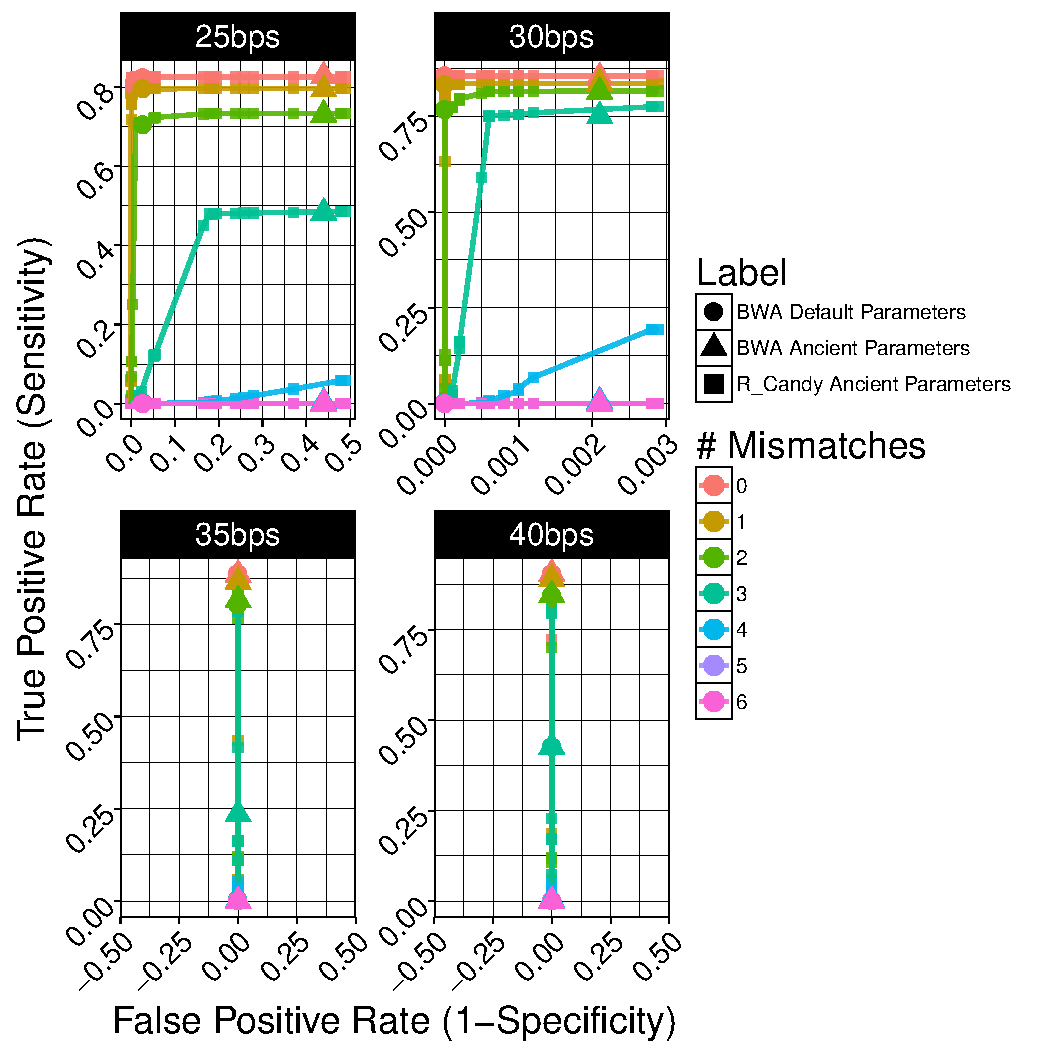
\includegraphics[width=11cm]{pictures/f_DS9_22_20_54_emp.pdf}
\caption{ 
ROC curve for the alignment to the human reference genome of simulated 
fresh sequence reads with ancient parameters. See Section \ref{Evaluation 
Scenarios} for more details.
}
\label{DS9_emp}
\end{figure}
 

The result of aligning fresh DNA reads extracted from the human genome
to the human reference genome (Figure \ref{DS9_emp})confirms the result 
of the similar test of aligning fresh DNA extracted from simulated genome 
to the simulated genome.  

 
Results show a big specificity difference between length 25 bps and 30 bps, 
where increasing the length decreases the rate of spurious alignments of
exogenous reads. However, it shows an improvement of no false positive (spurious
alignments of contaminant exogenous reads) for longer reads of length 35 bps and 
40 bps for R-Candy and BWA either default or ancient parameters. 

As is expected, increasing the number of mismatches ( increased divergence ) 
decreases the sensitivity of both aligners. A huge decrease in specificity is
illustrated which introducing 3 mismatches to the reads which simulates a very
high divergence rate of 12\% and 10\% for lengths 25 bps and 30 bps respectively.


%%%%%%%%%%%%%%%%%%%%%%%%%%%%%%%%%%%%%%%%%%%%%%%%%%%%%%%%%%%%%%%%%%%%%%%%%%%%%%%%

\subsection{Evaluation on Simulated Ancient DNA Reads}

\subsubsection{Alignment of Simulated Ancient DNA Reads to a Simulated Genome.}
\label{ Alignment of Simulated Ancient DNA Reads to a Simulated Genome.}

\begin{itemize}
 
   
    \item \textbf{Data:} Simulated ancient DNA 
     with ancient parameters (deamination damage, $ \sigma = 0.9$, 
    $ \sigma' = 0.93 $, $\delta = 0.02 $,  and $p = 0.3 $ \cite{mapdamage2})
    and between 0 and 6 substitutions to allow increasing sequence divergence
    and on top of them sequencing error generated from empirical quality 
    distribution data extracted from a simulated genome.
  
 
   \item \textbf{Reference genome:}  Reads were aligned to a simulated genome of 
   length 1 Gb.


  \item \textbf{Aligners:} R-Candy with ancient parameters 
  (deamination damage, -l left overhang parameter= 0.3,
   -r right overhang parameter= 0.3 , 
   -d deamination rate in double stranded section = 0.02 , 
   -s deamination rate in single stranded section = 0.9 )
   and cutoff for alignment score at 20. \\
   BWA with default parameters and ancient parameters \cite{green2010draft}
   (mismatch parameter -n set to 0.01 and the number of gap openings -o
   to 2)

  \end{itemize}


Here we aim to evaluate the performance of R-Candy on ancient DNA reads with 
deamination parameters.


\begin{figure}[H]
\centering
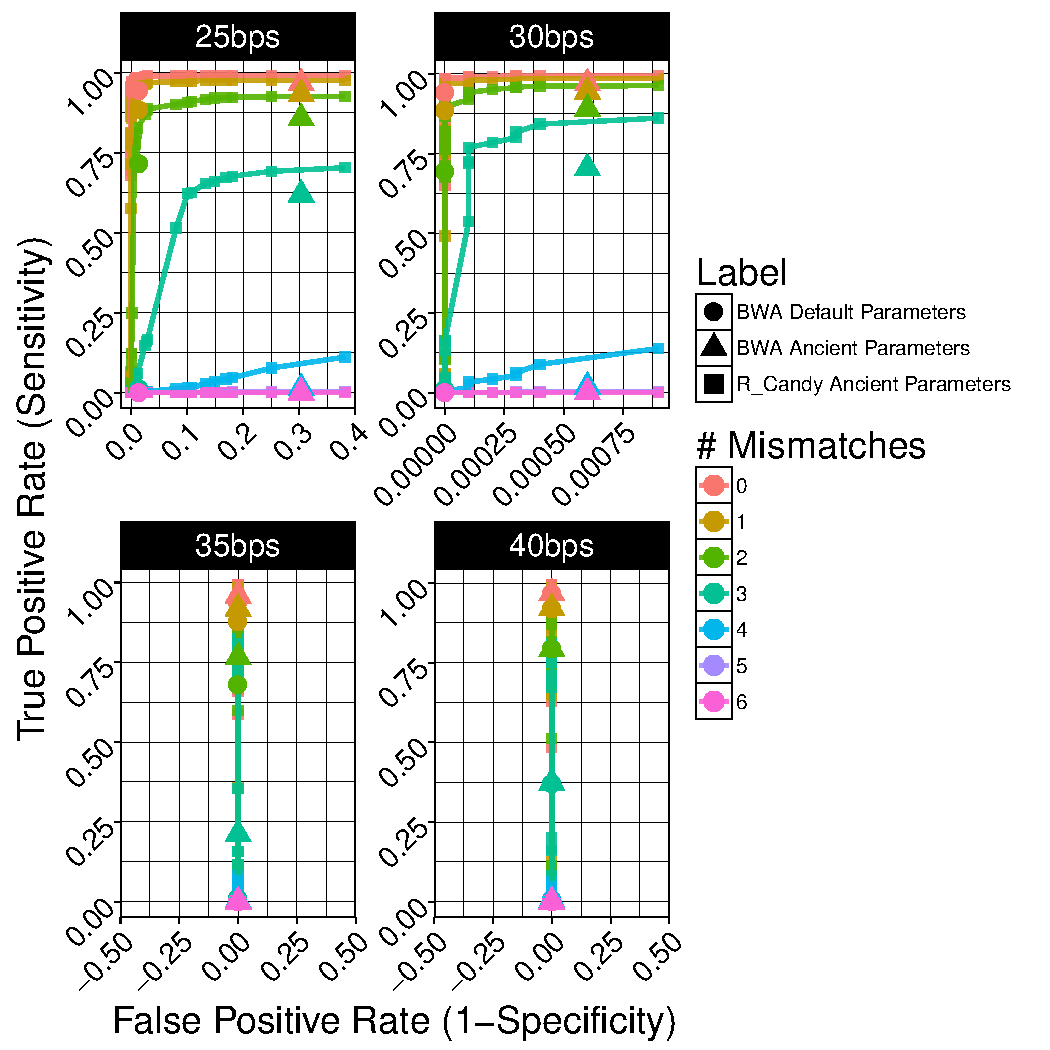
\includegraphics[width=12cm]{pictures/f_DS1_emp.pdf}

\caption{
ROC curve for the alignment to the simulated reference genome of simulated ancient
sequence reads. See Section \ref{Evaluation Scenarios} for more details.}
\label{DS1_emp}
\end{figure}


As the result shows (Figure \ref{DS1_emp}), R-Candy achieves the highest rate of
sensitivity in all four given lengths.

Reads in length 25 are very challenging for aligners, where the spurious 
alignments of contaminant read sequences are very likely.

For deaminated reads of length 25 bps with no divergence substitution (the plot
with zero mismatches), the sensitivity rate for R-Candy is 99\% compare to BWA 
with ancient-parameters 97\% and BWA with default parameters 94\%. 


For the reads of length 30 bps, the sensitivity values are 98\%, 94\% and 88\%
for R-Candy, BWA with ancient data parameters and BWA with default parameters
respectively, which again yields R-Candy's higher accuracy.

As is expected, introducing extra mismatches to the reads decreases  
the sensitivity of both aligners.

The huge decrease in the false positive rates between reads of length 25 bps and
30 bps show that even five bases difference can make a huge difference in the 
number of mapped exogenous reads.


No difference in specificity for reads longer than 35 bps is observed (no exogenous 
reads align).

BWA achieves higher sensitivity for short ancient read alignments when using the 
ancient parameters. However, with the inclusion of the deamination parameters 
R-Candy outperforms BWA in all cases.



 %%%%%%%%%%%%%%%%%%%%%%%%%%%%%%%%%%%%%%%%%%%%%%%%%%%%%%%%%%%%%%%%%%%%%%%


\subsubsection{Alignment of Simulated Ancient DNA Reads to the Human Reference Genome.}
\label{Alignment of Simulated Ancient DNA Reads to the Human Reference Genome.}
 
 \begin{itemize}
 
    \item \textbf{Data:} Simulated ancient DNA 
     with ancient parameters (deamination damage parameters, $ \sigma = 0.9$, 
    $ \sigma' = 0.93 $, $\delta = 0.02 $,  and $p = 0.3 $ and 
    between 0 and 6 substitutions to allow increasing sequence divergence
    including sequencing error generated from empirical quality distribution data
    extracted from a simulated genome.
  
   \item \textbf{Reference genome:} aligned to a the human reference genome (version hg19).

 
    \item \textbf{Aligners:} 
R-Candy with ancient parameters 
(deamination ancient parameters as -l left overhang parameter= 0.3, -r 
right overhang parameter= 0.3 , 
-d deamination rate in double stranded section = 0.02 , 
-s deamination rate in single stranded section = 0.9 )
and alignments score cut-off of 20. \\
BWA version 0.5.10-evan.10 with default parameters and ancient parameters 
(the mismatch parameter set to 0.01 
and the number of gap opens to 2)\cite{green2010draft}.
 
  \end{itemize}
 

Here we aim to evaluate the performance of R-Candy on ancient DNA reads, 
aligned to the human reference genome with the deamination parameters.


\begin{figure}[H]
\centering
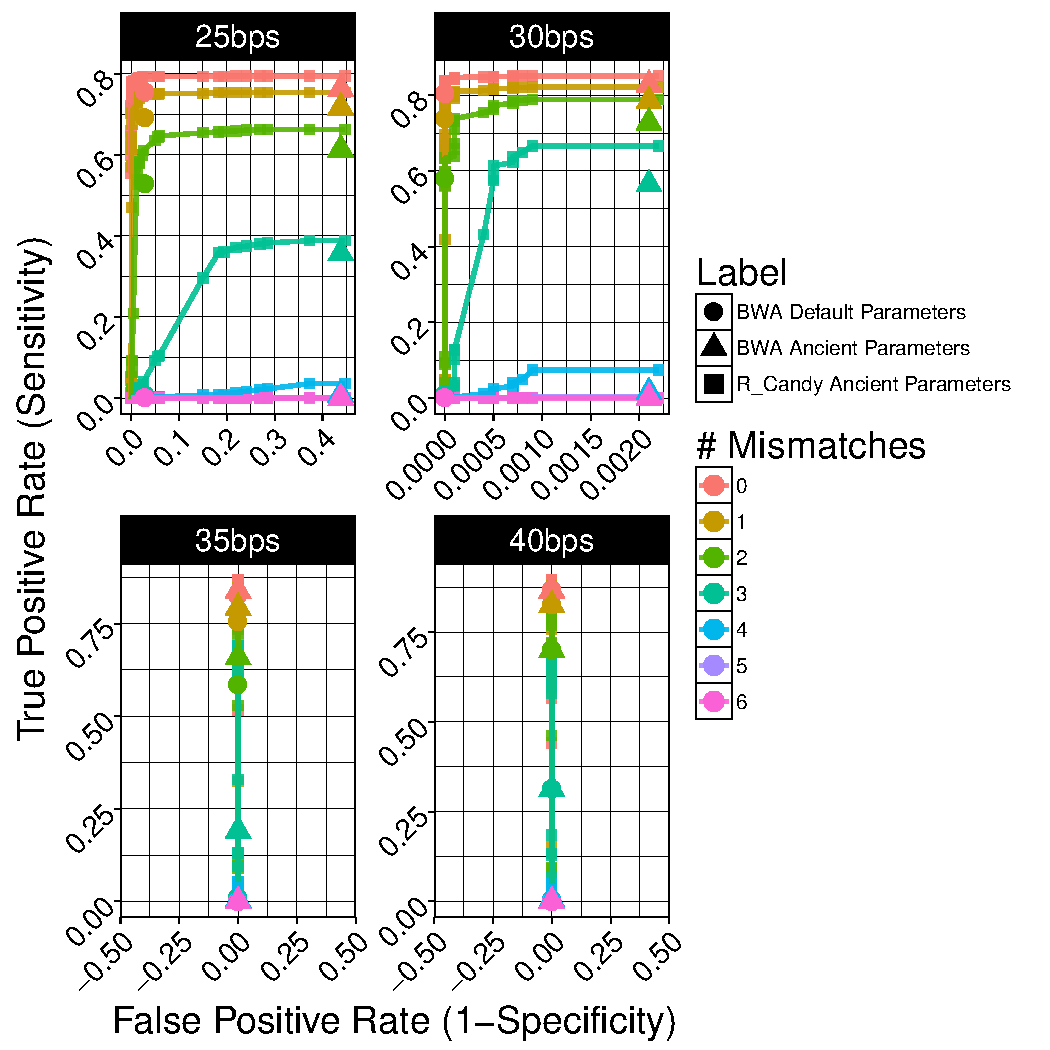
\includegraphics[width=12cm]{pictures/f_DS4_emp.pdf}

\caption{
ROC curve for the alignment to the human reference genome of simulated ancient
sequence reads. See Section \ref{Evaluation Scenarios} for more details.
}

\label{DS4_emp}
\end{figure}



The result of aligning ancient DNA reads extracted from the human genome and 
aligned back to the human genome (Figure \ref{DS4_emp})confirms the result of 
the similar test done on the Scenario 3, but with the lower sensitivity value 
due to the repetitive elements and other unknown characteristics of the human 
reference genome.

The lower sensitivity values for reads with higher simulated rate of divergence 
(simulated by a massive increase in the introduced differences to the reads) for
both R-Candy and BWA is observed in the results.

The highest specificity value for reads of length 25 bps shows the higher chance
of spurious alignments of contaminant reads for alignment of ultra-short reads.
So increasing the length of the reads leads to lower spurious alignment of 
exogenous read data.

The plots show no spurious alignments of contaminant exogenous reads of lengths 
bigger than 35 bps with specificity value of zero.

R-Candy with deamination parameters outperforms BWA in aligning ancient short DNA
reads to the human genome, although BWA provides more accurate alignments of short 
ancient reads when using the ancient parameters. 
 

%%%%%%%%%%%%%%%%%%%%%%%%%%%%%%%%%%%%%%%%%%%%%%%%%%%%%%%%%%%%%%%%%%%%%%%%%%%%%%%%%%%%%%%%%%


\subsection{Suitable Alignment Score} 
\label{Suitable Alignment Score}

We are looking for the best alignment score cutoff to achieve the 
highest accuracy (high sensitivity and specificity) while speeding 
up R-Candy's alignment process.

Using our simulation, we were looking for an alignment score that 
gives us a higher sensitivity than BWA with \quotes{ancient} parameters 
and better specificity than BWA with default parameters.
Which gives us the full sensitivity and complete benefit of rejecting
exogenous reads. 

Using the test scenario 4, aligning ancient reads to the human
genome for reads of length 30 bps and one mismatch (equivalent to 4\% 
divergence rate), at alignment score of range 12-13 of R-Candy 
achieves the higher accuracy (both higher sensitivity and 
specificity) compared to BWA with either default or \quotes{ancient} 
parameters.

Alignment score 12 is picked up as a suitable cutoff for R-Candy aligner. 

%%%%%%%%%%%%%%%%%%%%%%%%%%%%%%%%%%%%%%%%%%%%%%%%%%%%%%%%%%%%%%%%%%%%%%%%%%%%%%%%%%%%%%%%%%%

\subsection{Performance} \label{Performance}

The speed evaluation was done on small data sets of 3500 simulated ancient 
genomic and 1000 simulated ancient exogenous read sequences extracted from
the human genome and aligned back to the human reference genome of size 3.2 
Gbps by R-Candy and BWA aligners.
Table \ref{speed-RG} shows the speed and memory usage of R-Candy and BWA on 
the small data set. Both aligners ran on a single CPU. 
R-Candy ran with alignment score cutoff of 12 and 4 as the maximum
number number of hits to output per read. BWA also reports up to four
alignments and picks one as a best hit.  Notice that the time required for
building the genome index is not included in the reported time.\\

\begin{table}[H]
  \begin{tabular}{ |  p{2cm} | p{2cm} | p{2cm} | p{2cm} |p{2cm} | }
    \hline
  	\textbf{Type} & \textbf{Read length }&\textbf{Speed BWA  
  		default (no. of reads/s) }
  	&\textbf{Speed BWA ancient (no. of reads/s)} 
  	& \textbf{Speed R-Candy ancient (no. of reads/s)}\\ \hline
 	  Genomic    & 25  & 222 &  34   &  1.79 \\ \hline
      Genomic    & 30  & 526 &  52   &  2.22 \\ \hline
      Genomic    & 35  & 625 &  434   &  2.26 \\ \hline
 	  Genomic	 & 40  & 500 &  357   &  2.45 \\ \hline
 	  exogenous  & 25  & 147 &  13   &  1.68 \\ \hline
      exogenous  & 30  & 217 &  42   &  2.19 \\ \hline
 	  exogenous  & 35  & 232 &  153   &  1.67 \\ \hline
 	  exogenous  & 40  & 178 &  144   &  3.10 \\ \hline
   \end{tabular}
\caption{The alignment speed for ancient reads aligned to 
the human reference genome.}
\label{speed-RG}
\end{table}



The alignment of genomic reads of length 30 bps by BWA with \quote{ancient}
parameters (Table \ref{speed-RG}) is 23 times faster than alignment by R-Candy
with damage parameters.  

The throughput of both aligners is affected by the read length. The longer the
reads get the faster alignment we get. But BWA speed decrease at length 40 bps 
as BWA allows one more mismatch at this length.

The speed performance reveals on data sets of the size generated during ancient 
human studies projects (e.g. to align a run of one billion ancient reads of length
35 bps, R-Candy needs $\simeq $ 28 years while BWT ancient requires $\simeq 21$
days) R-Candy is therefore currently too slow for application to typical ancient 
DNA datasets.


\begin{table}[H]
  \begin{tabular}{ |  p{2cm} | p{2cm} | p{2cm} | p{2cm} |p{2cm} | }
    \hline
  	\textbf{Type} & \textbf{Read length }&\textbf{ BWA  
  		default memory usage (MB) }
  	&\textbf{ BWA ancient memory usage (MB) )} 
  	& \textbf{R-Candy memory usage (MB) }\\ \hline
 	  Genomic    & 25  & 945 &  947   &  1181 \\ \hline
      Genomic    & 30  & 945 &  949  &  1182 \\ \hline
      Genomic    & 35  & 945 &  945   &  1183 \\ \hline
 	  Genomic	 & 40  & 945 &  945   &  1181 \\ \hline
 	  exogenous  & 25  & 945 &  947   &  814 \\ \hline
      exogenous  & 30  & 945 &  947   &  815 \\ \hline
 	  exogenous  & 35  & 945 &  945   &  825 \\ \hline
 	  exogenous  & 40  & 945 &  945   &  828 \\ \hline
   \end{tabular}
\caption{The alignment speed for ancient reads aligned to 
the human reference genome.}
\label{speed-RG}
\end{table}

Both aligners show comparably efficient memory footprints.




%%%%%%%%%%%%%%%%%%%%%%%%%%%%%%%%%%%%%%%%%%%%%%%%%%%%%%%%%%%%%%%%%%%%%


\section{Conclusions} \label{Conclusions}


We have evaluated R-Candy, a novel method for aligning ancient DNA sequences.
The algorithm for scoring is based on a probabilistic model that takes into account 
the specific characteristics of ancient data, post-mortem deamination damage, as 
well as the other properties specific to the data, sequencing error, and species
divergence rate. 
\\
For both evaluated aligners, varying the cutoff (number of mismatches for BWA 
and alignment score for R-Candy) allows trading a slight increase in sensitivity 
for specificity and run time.
\\\\
The accuracy of R-Candy on aligning fresh DNA with "default" parameters (no damage model) 
matches BWA, with either "default" or "ancient" parameters, depending  on the cutoff values.
\\\\
R-Candy has a higher sensitivity value on aligning ancient DNA with ancient parameters
compared to BWA with "ancient" parameters and better specificity compared to the 
"default" BWA at the alignment score cutoff value of 12.
\\\\
The accuracy of R-Candy on aligning fresh DNA with "ancient" parameters
(deamination damage model) matches BWA, with either "default" or "ancient" 
parameters, depending  on the cutoff values.
\\\\
In terms of memory footprint, both aligners are equally good and memory efficient
to load genome. But R-Candy has a very low throughput ratio (speed) compared to 
BWA which makes it unusable in case of big-data and genome of mammalian size. 
\\\\
The main conclusion is that R-Candy reduces the minimum read length needed
for aDNA alignment from 35 bps to about 25 bps, which makes it possible to
align more rare and low-quality endogenous reads, and also R-Candy can be 
used as a part of a sensible workflow in ancient DNA studies working with all 
types of DNA (ancient and fresh). But some modifications are needed to 
increase its alignment speed in order to be useable on data sets of the
size typically generated during ancient human genome sequencing projects. 



 
%%%%%%%%%%%%%%%%%%%%%%%%%%%%%%%%%%%%%%%%%%%%%%%%%%%%%%%%%%%%%%%%%%%%%%

\section{Future Work} \label{Future Work}


We have shown that for the alignment of ancient DNA reads between 25-40 
bps, R-Candy provides superior accuracy to BWA. However, a number of points 
need to be addressed before R-Candy can be used on big data sets of ancient
genome projects. 

%To increase R-Candy's speed  ...

The backtracking algorithm used by R-Candy is its bottleneck if mismatches 
appear early in the alignment. The middle part of a read is the least
affected by deamination damage in ancient DNA read sequences,
therefore, alignment of aDNA reads should start from the middle of the 
read out, which requires a different index structure (Bi-directional Wavelet 
Tree). This would also enable a seed strategy, where the middle part of a read
would serve as seed.

As mentioned before\ref{Bi-directional Wavelet Index} the requirement for new index
structure (Bi-directional Wavelet Tree index) is already in the code just
needs some modification to be used as a bi-directional index structure. 
But there is a need for a different searching algorithm to start from the 
middle part of the ancient reads and aligns in both directions to be implemented.


Make the program parallel and support distributed computing feature
speeds up the software by dividing a computational job into many tasks 
and solve each task by one or more computers or CPUs.

A method that combines dynamic programming with a Full-Text index might 
extend the usefulness of R-Candy to longer reads.

%%%%%%%%%%%%%%%%%%%%%%%%%%%%%%%%%%%%%%%%%%%%%%%%%%%%%%%%%%%%%%%%%%%%%%

\section{Availability} \label{Availability}

R-Candy's documentation and source code as a Haskell program are freely
available at\\
 (https://bitbucket.org/ustenzel/r-candy.
\\\\
Genome/read simulation program written in C++ is freely available at
(https://github.com/Homa1127/simulateGenome.git).
\\\\
The hash program for analysing R-Candy's output written in C++, available at
https://github.com/Homa1127/rcandyHash.git



%%%%%%%%%%%%%%%%%%%%%%%%%%%%%%%%%%%%%%%%%%%%%%%%%%%%%%%%%%%%%%%%%%%%%%%%

\section{Abbreviations} \label{Abbreviations}

\textbf{DNA}: deoxyribonucleic acid;
\textbf{bp}: base pair;
\textbf{NGS}: next generation sequencing technologies;
\textbf{BWT}: Burrows-Wheeler transform;
\textbf{FM}: full-text minute-space;
\textbf{A}: Adenine;
\textbf{C}: Cytosine;
\textbf{T}: Thymine;
\textbf{G}: Guanine;
\textbf{CpG}: C followed by G;
\textbf{SA}: suffix array;
\textbf{LF}: last to first;
\textbf{DFS}: depth first search;
\textbf{DP}: dynamic programming;
\textbf{BAM}: Binary Alignment/Map;
\textbf{CDF}: cumulative distribution function.
\textbf{PCR}: Polymerase Chain Reaction.



%%%%%%%%%%%%%%%%%%%%%%%%%%%%%%%%%%%%%%%%%%%%%%%%%%%%%%%%%%%%%%%%%%%%%

\newpage
\appendix
\section*{Appendix}
\renewcommand{\thesubsection}{\Alph{subsection}}

\subsection{Simulation of sequencing error by ART software} 
\label{Simulation sequencing error by ART software}

In this section, I follow all the evaluation scenarios which I explained in
Section \ref{Evaluation Scenarios}  with different sequencing error simulation.
ART \cite{art}, a next-generation sequencing read simulator is used to simulate sequencing
error of Illumina platform. 
ART generates sequencing reads based on different sequencing technology 
platforms (454, Illumina, SOLiD) criteria \cite{art} and simulates the
substitution error probability, based on the base-quality 
score distribution reported by large training data sets \cite{art}.\\

In order to use ART in readSim, the user needs to specify the sequencing
platform and the read length for generating base quality scores.\\

The result of aligning different data sets showed that ART simulates a
low base quality (compared to the empirical data) that leads to 
a high rate of sequencing error which degrades the performance of BWA.\\
Therefore the result of ART simulation is not used in this evaluation. \\

As the result shows R-Candy performs well with a high sensitivity rate 
even with a high rate of sequencing error while BWA collapses catastrophically.\\

\begin{figure}[H]
\centering
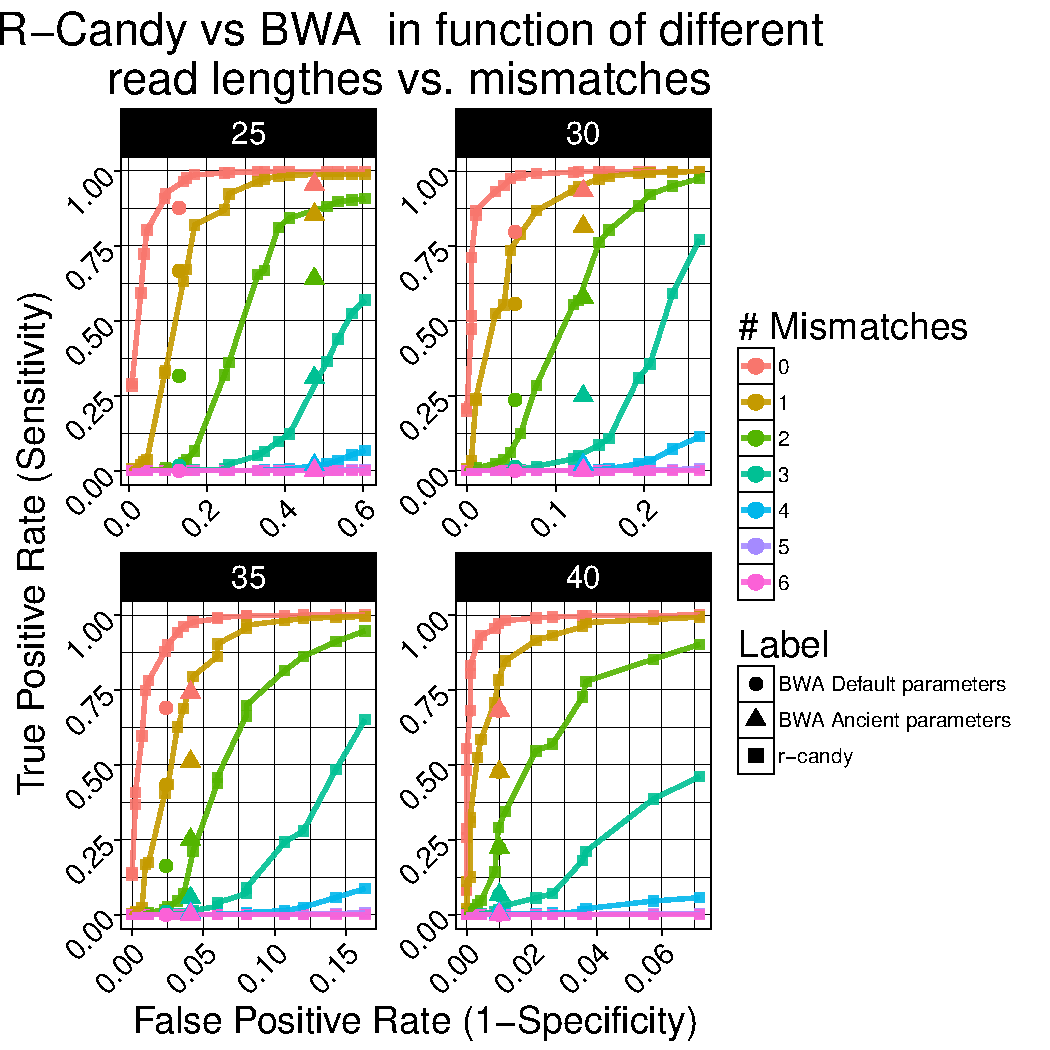
\includegraphics[width=12cm]{pictures/bROC_DS3_ART.pdf}
\caption{
ROC curve for the alignment to the simulated reference genome of simulated fresh 
sequence reads of lengths 25-40 bps with between 0 and 6 substitutions due 
to increasing sequence divergence and sequencing error by ART.}
\label{DS3_ART}
\end{figure}



\begin{figure}[H]
\centering
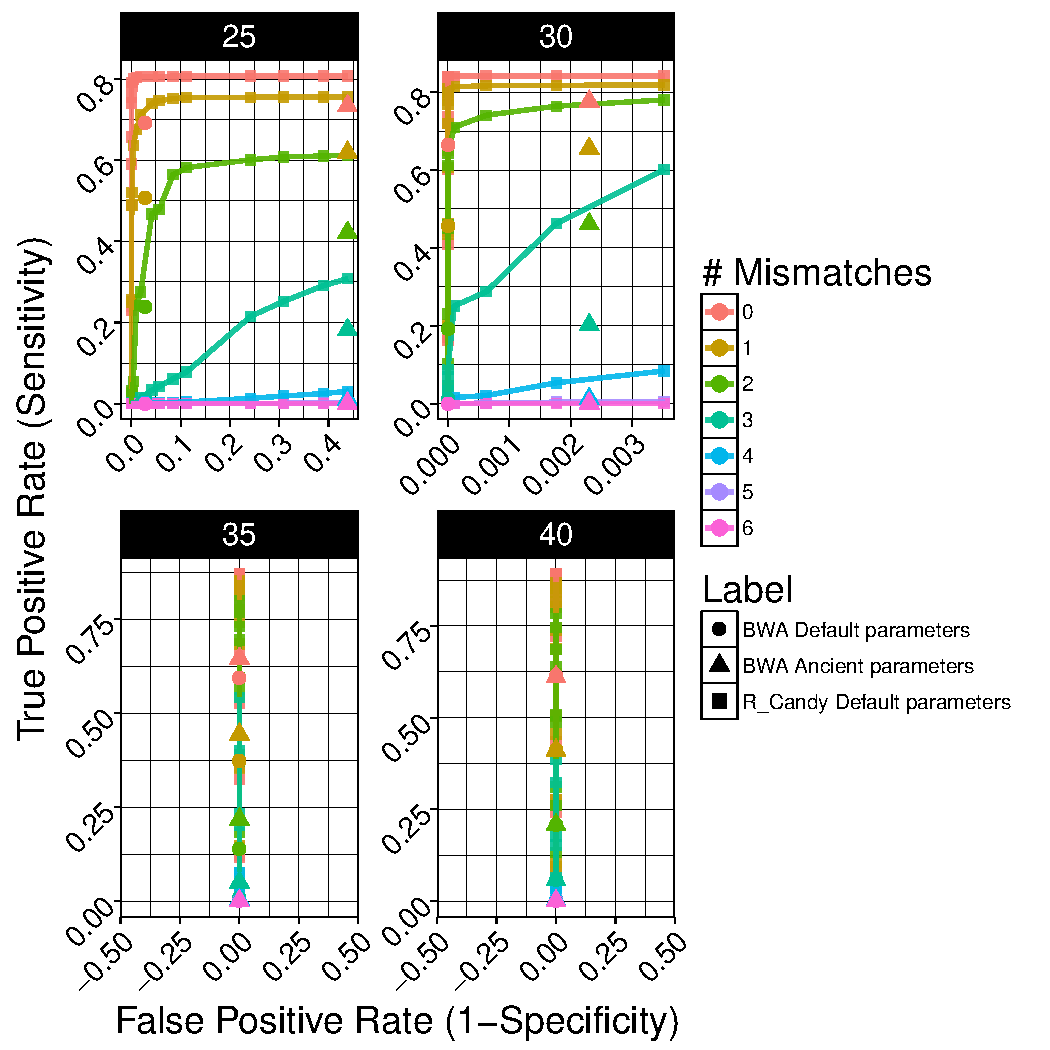
\includegraphics[width=12cm]{pictures/bROC_DS6_ART.pdf}
\caption{
ROC curve for the alignment to the human reference genome of simulated fresh 
sequence reads of lengths 25-40 bps with between 0 and 6 substitutions due 
to increasing sequence divergence and sequencing error by ART.
}
\label{DS6_ART}
\end{figure}



\begin{figure}[H]
\centering
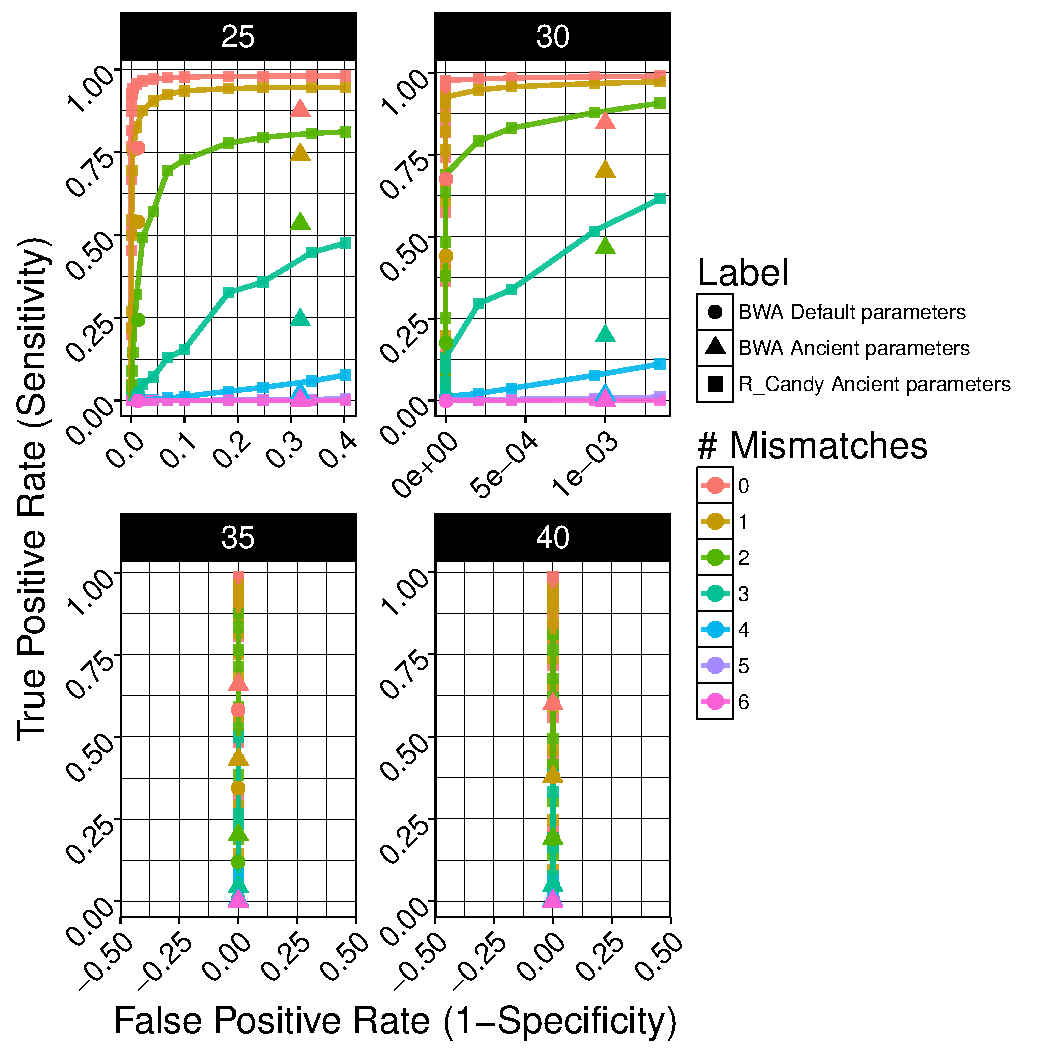
\includegraphics[width=12cm]{pictures/bROC_DS1_ART.pdf}
\caption{
ROC curve for the alignment to the simulated reference genome of simulated ancient 
sequence reads of lengths 25-40 bps with ancient parameters as explained in Data 
and between 0 and 6 substitutions due to increasing sequence divergence and
empirical sequencing error.
}
\label{DS1_ART}
\end{figure}



\begin{figure}[H]
\centering
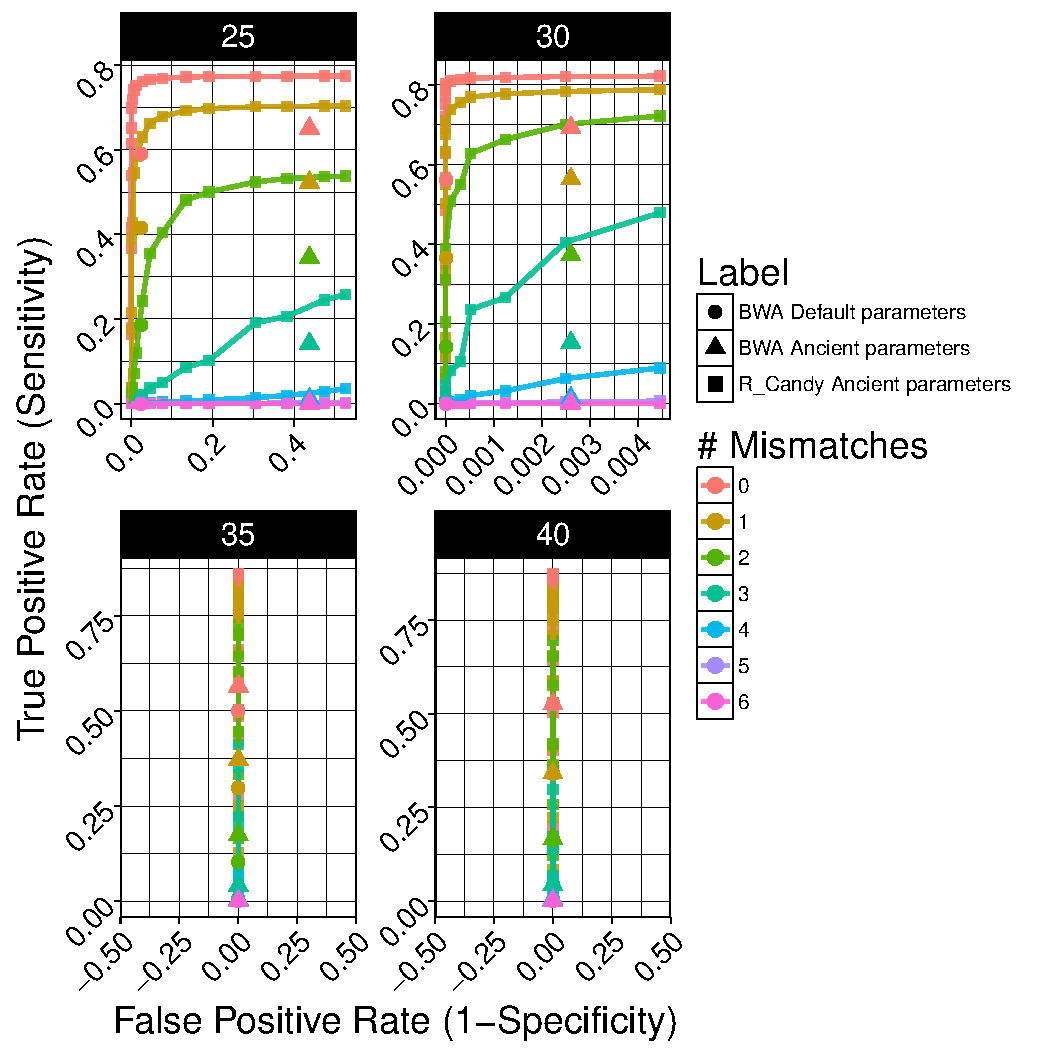
\includegraphics[width=12cm]{pictures/bROC_DS4_ART.pdf}
\caption{
ROC curve for the alignment to the human reference genome of simulated ancient 
sequence reads of lengths 25-40 bps with ancient parameters as explained in Data 
and between 0 and 6 substitutions due to increasing sequence divergence and
empirical sequencing error.
}
\label{DS4_ART}
\end{figure}



%%%%%%%%%%%%%%%%%%%%%%%%%%%%%%%%%%%%%%%%%%%%%%%%%%%%%%%%%%%%%%%%%%%%
\bibliographystyle{unsrt}
\bibliography{Ref}


\end{document} 
   
      
      
              
